\documentclass{beamer}
\usepackage{amsmath,amsbsy,amsopn,amstext,amsfonts,amssymb}
\usepackage{isomath}
\usepackage{ulem}
%\linespread{1.6}  % double spaces lines
\usepackage{graphicx}
\usepackage{subfigure}
\usepackage{color}
\usepackage{optidef}  % define optimization problems
\usepackage{multicol}  % multiple columns
\usepackage{listings} % for python code
\usepackage{mathrsfs}

\usepackage{polynom}
\newcommand{\adj}{\mathrm{adj}}
\newcommand{\constrainedmin}[3]{
		\begin{mini*}|s|
		{#2}{#1}{}{}
		\addConstraint{#3}
		\end{mini*}
}

\newcommand{\rwbcomment}[1]{{\color{blue}RWB:#1}}
\newcommand{\defeq}{\stackrel{\triangle}{=}}
\newcommand{\abs}[1]{\left|#1\right|}
\newcommand{\norm}[1]{\left\|#1\right\|}
\newcommand{\iprod}[1]{\left<#1\right>}
\newcommand{\ellbf}{\boldsymbol{\ell}}
\newcommand{\nubf}{\boldsymbol{\nu}}
\newcommand{\mubf}{\boldsymbol{\mu}}
\newcommand{\abf}{\mathbf{a}}
\newcommand{\bbf}{\mathbf{b}}
\newcommand{\cbf}{\mathbf{c}}
\newcommand{\dbf}{\mathbf{d}}
\newcommand{\ebf}{\mathbf{e}}
\newcommand{\fbf}{\mathbf{f}}
\newcommand{\gbf}{\mathbf{g}}
\newcommand{\hbf}{\mathbf{h}}
\newcommand{\ibf}{\mathbf{i}}
\newcommand{\jbf}{\mathbf{j}}
\newcommand{\kbf}{\mathbf{k}}
\newcommand{\lbf}{\mathbf{l}}
\newcommand{\mbf}{\mathbf{m}}
\newcommand{\nbf}{\mathbf{n}}
\newcommand{\obf}{\mathbf{o}}
\newcommand{\pbf}{\mathbf{p}}
\newcommand{\qbf}{\mathbf{q}}
\newcommand{\rbf}{\mathbf{r}}
\newcommand{\sbf}{\mathbf{s}}
\newcommand{\tbf}{\mathbf{t}}
\newcommand{\ubf}{\mathbf{u}}
\newcommand{\vbf}{\mathbf{v}}
\newcommand{\wbf}{\mathbf{w}}
\newcommand{\xbf}{\mathbf{x}}
\newcommand{\ybf}{\mathbf{y}}
\newcommand{\zbf}{\mathbf{z}}
\newcommand{\Jbf}{\mathbf{J}}
\newcommand{\Acal}{\mathcal{A}}
\newcommand{\Bcal}{\mathcal{B}}
\newcommand{\Lcal}{\mathcal{L}}
\newcommand{\Ncal}{\mathcal{N}}
\newcommand{\Rcal}{\mathcal{R}}
\definecolor{darkolivegreen}{rgb}{0.33, 0.42, 0.18}

\makeatletter
\newenvironment<>{proofstart}[1][\proofname]{%
    \par
    \def\insertproofname{#1\@addpunct{.}}%
    \usebeamertemplate{proof begin}#2}
  {\usebeamertemplate{proof end}}
\newenvironment<>{proofcont}{%
  \setbeamertemplate{proof begin}{\begin{block}{}}
    \par
    \usebeamertemplate{proof begin}}
  {\usebeamertemplate{proof end}}
\newenvironment<>{proofend}{%
    \par
    \pushQED{\qed}
    \setbeamertemplate{proof begin}{\begin{block}{}}
    \usebeamertemplate{proof begin}}
  {\popQED\usebeamertemplate{proof end}}
\makeatother

\title{ECEn 671: Mathematics of Signals and Systems \\ 
Moon: Chapter 4.}
\author{Randal W. Beard}
\institute{Brigham Young University}
\date{\today}

\begin{document}

%-------------------------------
\begin{frame}
	\titlepage
\end{frame}

%-------------------------------
\begin{frame}[t]
\frametitle{Table of Contents}
\tableofcontents
\end{frame}

%%%%%%%%%%%%%%%%%%%%%%%%%%%%%%%%%%%%%%%%%%%%%%%%%%%%%%%%%%%%%%%%%
\section{Linear Operators}
\frame{\sectionpage}


%----------------------------------
\begin{frame}\frametitle{Linear Operators}
	Recall from Chapter~3 the definition of a Linear operator:  
	\begin{definition}
	Let $\mathbb{X}$ and $\mathbb{Y}$ be vector spaces, then $\mathcal{A}:\mathbb{X} \to \mathbb{Y}$ is a linear operator if
	\[ 
	\mathcal{A}[\alpha_1 x_1 + \alpha_2 x_2 ] = \alpha_1 \mathcal{A}[x_1] + \alpha_2 \mathcal{A}[x_2] 
	\]	
	$\forall x_1,x_2 \in \mathbb{X}$ and $\forall \alpha_1,\alpha_2 \in \mathbb{F}$
	\end{definition}
	
	\vfill
	See chapter 2 notes (slides 79--83) for examples of linear operators.
\end{frame}

%----------------------------------
\begin{frame}\frametitle{Norm of a Linear Operator}
	An important concept is the \underline{norm} of an operator.  There are several ways to define norms for operators.  The most important is the ``induced'' or ``subordinate'' norm.
	
	\vfill
	
	\begin{definition}
		Let $\mathcal{A}:\mathbb{X} \to \mathbb{Y}$ then
		\begin{align*}
		\norm{\mathcal{A}} &= \sup_{x \neq 0} \frac{\norm{\mathcal{A}[x]}_{\mathbb{Y}}}{\norm{x}_{\mathbb{X}}} \\
		&= \sup_{\norm{x}_{\mathbb{X}}=1} \norm{\mathcal{A}[x]}_{\mathbb{Y}} 
		\end{align*}
	\end{definition}
	
	\vfill
	
	Different norms on $\mathcal{A}$ are defined by taking different norms in $\mathbb{X}$ and $\mathbb{Y}$.
\end{frame}

%----------------------------------
\begin{frame}\frametitle{Norm of a Linear Operator, Examples}
	\begin{example}
	Let $\mathcal{A}: L_2 \to L_2$ then
	\begin{align*}
	\norm{\mathcal{A}}_2 &= \sup_{x \neq 0} \frac{\norm{\mathcal{A}[x]}_{L_2}}{\norm{x}_{L_2}} \\
	&= sup_{\norm{x}_{L_2} = 1} \norm{\mathcal{A}[x]}_{L_2} 
	\end{align*}
	\end{example}
	
	\begin{example}
		Let $\mathcal{A}: L_{\infty} \to L_{\infty}$ then
		\begin{align*}
			\norm{\mathcal{A}}_{\infty} &= \sup_{x \neq 0} \frac{\norm{\mathcal{A}[x]}_{L_{\infty}}}{\norm{x}_{L_{\infty}}} \\
			&= \sup_{\norm{x}_{L_{\infty}} = 1} \norm{\mathcal{A}[x]}_{L_{\infty}}
		\end{align*}
	\end{example}
\end{frame}

%----------------------------------
\begin{frame}\frametitle{Norm of a Linear Operator, Examples}
	\begin{example}
	Let $\mathcal{A}: L_p \to L_p$ then
	\begin{align*}
		\norm{\mathcal{A}}_p &= \sup_{x \neq 0} \frac{\norm{\mathcal{A}[x]}_{L_p}}{\norm{x}_{L_p}} \\
		&= \sup_{\norm{x}_{L_p} = 1} \norm{\mathcal{A}[x]}_{L_p} 
	\end{align*}
	\end{example}

	\vfill
	
	Why is it called the induced or subordinate norm?  The norm on the operator is induced by the vector norm.
\end{frame}

%----------------------------------
\begin{frame}\frametitle{Norm of a Linear Operator, Geometric Interpretation}
	\[ 
	\norm{A} = \sup_{\norm{x} = 1} \norm{Ax} 
	\]
	\begin{center}
		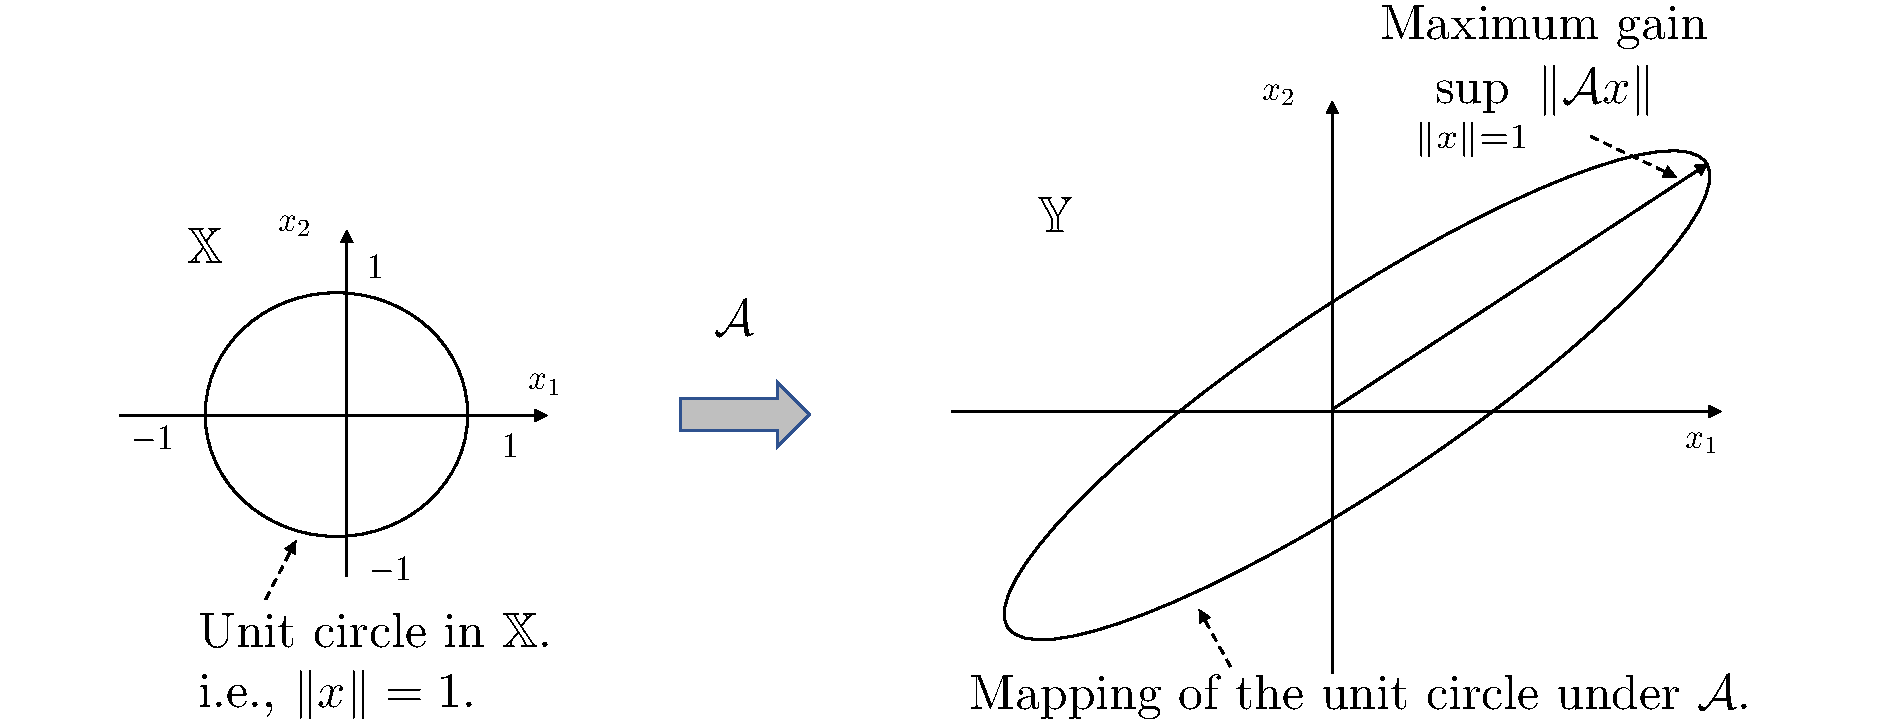
\includegraphics[width=4in]{figures/chap4_matrix_norm}	
	\end{center}
\end{frame}

%----------------------------------
\begin{frame}\frametitle{Norm of a Linear Operator, System Interpretation}
	Given a linear system
	\begin{center}
		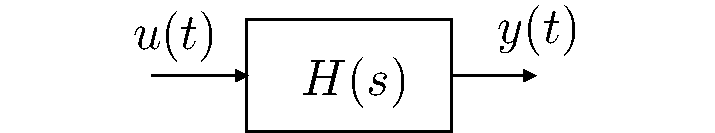
\includegraphics[width=2in]{figures/chap4_linear_system}	
	\end{center}

	\vfill
	
	The norm of the system $H(s)$ is the maximum gain of the system.
\end{frame}

%----------------------------------
\begin{frame}\frametitle{Norm of BIBO System}
	Let $\mathcal{A}: L_{\infty} \to L_{\infty}$ be an LTI system that is BIBO stable with impulse response $h(t)$, then
	\begin{align*}
	y(t) &= \int_0^t h(t-\tau)u(\tau)d\tau \\
		&\defeq \mathcal{A}[u] 
	\end{align*}
	
	\vfill
	
	Find $\norm{\mathcal{A}}_{\infty}$.
\end{frame}

%----------------------------------
\begin{frame}\frametitle{Norm of BIBO System, cont}
	\begin{lemma}
	\begin{align*}
	\norm{\mathcal{A}}_{\infty} &= \norm{h}_{L_1[0,\infty]} \\
		&\defeq \int_0^{\infty} |h(t)|dt 
	\end{align*}
	\end{lemma}
	
	\begin{proof}
		We need to prove two things
		\begin{enumerate}
		\item $\norm{\mathcal{A}}_{\infty} \leq \displaystyle\int_0^{\infty} |h(t)|dt$
		\item $\displaystyle\int_0^{\infty}|h(t)|dt \leq \norm{\mathcal{A}}_{\infty}$
		\end{enumerate}
	\end{proof}
\end{frame}

%----------------------------------
\begin{frame}\frametitle{Norm of BIBO System, Proof}
	\underline{Proof of 1.}

	\begin{align*}
		\sup_{\norm{x}_{\infty} = 1} \norm{\mathcal{A}[u]}_{\infty} &= \sup_{\norm{u}_{\infty} =
  		1} \norm{ \int_0^t h(t - \tau) u(\tau) d\tau  }_{\infty}
		\\
		&= \sup_{\norm{u}_{\infty} = 1} \left[ \sup_{t > 0} \abs{
  			\int_0^t h(t-\tau)u(\tau)d\tau} \right]\\
		&\leq \sup_{\norm{u}_{\infty} = 1} \left[ \sup_{t > 0}
  			\int_0^t \abs{ h(t-\tau)u(\tau)} d\tau \right]\\
		&\leq \sup_{\norm{u}_{\infty} = 1} \left[ \norm{ u }_{\infty} \sup_{t > 0} \int_0^t \abs{ h(t - \tau)} d\tau
			\right]\\
		&\leq \int_0^{\infty} \abs{h(\tau)}d\tau = \norm{h}_{L_1[0,\infty]}
	\end{align*}
\end{frame}

%----------------------------------
\begin{frame}\frametitle{Norm of BIBO System, Proof}
	\underline{Proof of 2.}
	
	Let $\hat{u}_t(\tau) = \begin{cases}
			1 & \text{ if } h(t-\tau) \geq 0\\
			-1 & \qquad \text{ otherwise }
			\end{cases}$.

	Note that $\norm{\hat{u}_t}_{\infty} = 1$ $\forall t>0$, we have that
	\[ 
		\int_0^t h(t-\tau)\hat{u}_t(\tau)d\tau = \int_0^t \abs{h(t - \tau)} d\tau.
	\]
	Therefore for this particular choice of $\hat{u}_t$ we have that
	\[ 
		\sup_{t > 0} \left[ \int_0^t \abs{h(t-\tau)}d\tau\right] = \norm{ A\hat{u}_\infty }_{\infty} = \int_0^{\infty} \abs{h(\tau)}d\tau.
	\]
	By definition of $\sup$
	\[ 
		\int_0^{\infty} \abs{h(\tau)}d\tau = \norm{ A\hat{u}_\infty }_{\infty} \leq
		\sup_{\norm{u}=1} \norm{Au}_{\infty}.
	\]
\end{frame}

%----------------------------------
\begin{frame}\frametitle{Operator Norm: Proof Technique}
	The proof technique shown here is the general approach to show that the norm of an operator is some value. 
	
	\vfill 

	Suppose that you would like to prove that
	\[ 
	\norm{\mathcal{A}} = M.
	\]
	You need to show two things
	\begin{enumerate}
		\item $\norm{\mathcal{A}} \leq M$
		\item $M \leq \norm{\mathcal{A}}$.
	\end{enumerate}
\end{frame}

%----------------------------------
\begin{frame}\frametitle{Operator Norm: Proof Technique}
	To show (1) use triangle and other inequalities to show that 
	\[ 
	\norm{\mathcal{A}x} \leq M\norm{x} 
	\]
	which implies that
	\[ 
	\sup_{\norm{x} = 1} \norm{\mathcal{A}x} \leq
		\sup_{\norm{x}=1} M\norm{x} = M 
	\]

	\vfill
	
	To show (2), construct a specific $\hat{x}$ such that
	\[ 
	\norm{ \hat{x} } = 1 \text{ and } \norm{ \mathcal{A}\hat{x} } = M.
	\]
	This implies that
	\[ 
		M \leq \sup_{\norm{x}=1} \norm{\mathcal{A}x} = \norm{\mathcal{A}}.
		\]	
\end{frame}

%----------------------------------
\begin{frame}\frametitle{Properties of Linear Operators}
	\begin{lemma}
		For any induced operator norm,
		\[ 
		\norm{\mathcal{A}x} \leq \norm{\mathcal{A}}\norm{x}. 
		\]
	\end{lemma}
	
	\begin{proof}
		\[ 
		\norm{\mathcal{A}} = \sup_{x \neq 0} \frac{\norm{\mathcal{A}x}}{\norm{x}}.
		\]
	Therefore for any $x \neq 0$ we must have that
	\begin{align*}
	&\norm{\mathcal{A}} \geq \frac{\norm{\mathcal{A}x}}{\norm{x}} \\
	\Rightarrow & \norm{\Acal x} \leq \norm{\mathcal{A}}\norm{x}.
	\end{align*}
	\end{proof}	
\end{frame}

%----------------------------------
\begin{frame}\frametitle{Properties of Linear Operators, cont}
	\begin{lemma}
		All induced operator norms satisfy the ``submultiplicative property,'' i.e.,
		\[ 
			\norm{\mathcal{A}\mathcal{B}} \leq \norm{\mathcal{A}}\norm{\mathcal{B}} 
			\]
	\end{lemma}
	
	\begin{proof}
		\begin{align*}
		\norm{\mathcal{A}\mathcal{B}} &= \sup_{\norm{x}=1}\norm{\mathcal{A}\mathcal{B}x} \\
				  &\leq \sup_{\norm{x} = 1} \norm{\mathcal{A}}\norm{\mathcal{B}x} \\
				  &\leq \sup_{\norm{x}=1}\norm{\mathcal{A}}\norm{\mathcal{B}}\norm{x} \\
				  &= \norm{\mathcal{A}}\norm{\mathcal{B}}
		\end{align*}
	\end{proof}
\end{frame}

%----------------------------------
\begin{frame}\frametitle{Properties of Linear Operators, cont}
	\begin{definition}
		An operator $\mathcal{A}:\mathbb{X}\to \mathbb{Y}$ is \underline{bounded} if
		$\norm{\Acal} < \infty$
	\end{definition}
	
	\vfill

	\begin{definition}
		The following three statements are equivalent
		\begin{enumerate}
			\item $\Acal:\mathbb{X}\to\mathbb{Y}$ is \underline{continuous}
			\item $x_n \to x^\ast \Rightarrow \Acal[x_n] \to \Acal[x^\ast] $ for all convergent sequences in $\mathbb{X}$
			\item $\forall \epsilon > 0, \quad \exists \delta > 0$ such that
				\[
				\norm{x - y} \leq \delta \quad \Rightarrow \quad \norm{ \Acal[x]-\Acal[y] } < \epsilon \qquad \forall x,y \in \mathbb{X} 
				\]
		\end{enumerate}
	\end{definition}
\end{frame}

%----------------------------------
\begin{frame}\frametitle{Properties of Linear Operators, cont}
	\begin{theorem}[Moon Theorem 4.1]
		A linear operator is bounded iff it is continuous.
	\end{theorem}

	\begin{proof}\end{proof}
	($\Rightarrow$) Suppose $\norm{ \Acal }=M < \infty$,let $\{x_n\}$ be any convergent sequence with limit $x^\ast\in\mathbb{X}$, then 
	\begin{align*}
	\norm{ \Acal x_n - \Acal x^\ast } &= \norm{ \Acal(x_n-x^\ast) } \leq \norm{ \Acal }\norm{x_n-x^\ast }\\
		&= M\norm{ x_n-x^\ast }\to 0 \Rightarrow \norm{\Acal x_n-\Acal x^\ast }\to 0.
	\end{align*}
	Therefore $\Acal$ is continuous.
	
\end{frame}

%----------------------------------
\begin{frame}\frametitle{Proof, cont}
	\noindent ($\Leftarrow$) Assume $\Acal$ is continuous and let $\epsilon = 1$ and $y = 0$ then $\exists \delta$ such that $\norm{ x } \leq \delta \Rightarrow \norm{ \Acal x } < 1$
	
	\vfill 

	Now let $0 \neq x \in \mathbb{X}$ be arbitrary, then 
	\[ 
	\norm{ \frac{\delta x}{\norm{ x }} } = \frac{\delta}{\norm{x}}\norm{ x } = \delta \leq \delta 
	\]
	implies that
	\[
		\norm{\Acal\left( \frac{\delta x}{\norm{ x }}\right)} = \frac{\delta}{\norm{ x }}\norm{ \Acal x } < 1
	\]
	which implies that
	\[
	\norm{ \Acal x } \leq \frac{1}{\delta}\norm{ x }
	\]
	
	\vfill
	
	Therefore $\Acal$ is bounded.
\end{frame}

%----------------------------------
\begin{frame}\frametitle{Properties of Linear Operators, cont}
	\begin{theorem}[Moon Theorem 4.2]
		Let $\Acal:\mathbb{X}\to\mathbb{Y}$ be a linear operator.  If $\mathbb{X}$ is a finite dimensional Hilbert space, then $\Acal$ is bounded.
	\end{theorem}
	
	\begin{proof}\end{proof}
		Let $\dim(\mathbb{X}) = n$ and let $\{p_1, \cdots p_n\}$ be an orthonormal basis for $\mathbb{X}$, then
		\[ 
		x = \sum_{k = 1}^n \iprod{ x,p_k} p_k
		\]
\end{frame}

%----------------------------------
\begin{frame}\frametitle{Proof, cont.}

	Define $D = \max\{ \norm{ \Acal p_1 }, \norm{\Acal p_2 }, \ldots, \norm{\Acal p_n}\}$ then
	\begin{align*}
		\norm{\Acal x} &= \norm{\Acal\left( \sum_{k=1}^n \iprod{ x,p_k} p_k\right) } \\
			&\leq \sum_{k=1}^n \abs{\iprod{ x,p_k}}\norm{\Acal p_k } \\
			&\leq D\sum_{k=1}^n \abs{\iprod{ x,p_k} } \\
			&\leq D \sum_{k=1}^n \norm{ x }\norm{ p_k } \qquad{(Caucy-Schwartz)}\\
			&= D n \norm{ x }  \\
	\end{align*}
	
	Therefore $\Acal$ is bounded.	
\end{frame}

%%%%%%%%%%%%%%%%%%%%%%%%%%%%%%%%%%%%%%%%%%%%%%%%%%%%%%%%%%%%%%%%%
\section{Neumann Expansion}
\frame{\sectionpage}

%----------------------------------
\begin{frame}\frametitle{Geometric Series}
	One of the most important series in analysis is the geometric series
	\[ 
	S = 1 + x + x^2 + \ldots = \sum_{i=0}^{\infty}x^i 
	\]
	Noting that 
	\begin{align*}
		& 1 + xS = 1 + x + x^2 + \ldots = S \\
		\Rightarrow \qquad & S(1-x) = 1 \\
	\end{align*}
	Therefore 
	\[
	S = \sum_{i=0}^{\infty} x^i = \frac{1}{1-x} = (1-x)^{-1} 
	\]

	\vfill
	
	The series converges if $|x| < 1$.
\end{frame}

%----------------------------------
\begin{frame}\frametitle{Geometric Series for Operators (Neumann Expansion)}
	For operators we have a similar expression:
	\begin{theorem}[Moon Theorem 4.3]
	Suppose $\norm{ \cdot }$ is a norm satisfying the submultiplicative property and $\norm{\Acal} < 1$.  Then $(I-\Acal)^{-1}$ exists and
	\begin{align*}
		(I-\Acal)^{-1} &= \sum_{i=0}^{\infty} \Acal^i 
			= I + \Acal + \Acal^2 + \Acal^3 + \ldots\\
		\text{ where } & \\
		\Acal^2 &= \Acal\Acal \\
		\Acal^3 &= \Acal\Acal^2 \\
		\Acal^k &= \Acal\Acal^{k-1}.
	\end{align*}
\end{theorem}
\end{frame}

%----------------------------------
\begin{frame}\frametitle{Neumann Expansion, Proof}
	Suppose that $(I-\Acal)^{-1}$ does not exist.  Then $\Ncal(I-A)$ is non-trivial.
	
	Therefore, $\exists x \neq 0$ such that 
	\begin{align*}
	(I-\Acal)x = 0 \quad &\iff \quad x = \Acal x \\
	&\iff \quad \norm{ x } = \norm{\Acal x } \leq \norm{ \Acal }\norm{ x } < \norm{ x },
	\end{align*}
	which is a contradiction.  
	
	\vfill
	
	Therefore $(I-\Acal)^{-1}$ exists.
\end{frame}

%----------------------------------
\begin{frame}\frametitle{Neumann Expansion, cont.}
	Note that $\norm{ \Acal^k } \leq \norm{ \Acal }^{k}$ since $\norm{ \cdot }$ satisfies the submultiplication property. 
	
	\vfill 
	
	Since $\norm{\Acal } < 1$
	\[ 
	\lim_{k\to \infty} \norm{ \Acal^k } = 0 \quad \iff \quad \lim_{k \to \infty}\Acal^k = 0 
	\]
	
	\vfill
	
	Note that
	\[ 
	(I - \Acal) ( I + \Acal + \Acal^2 + \cdots + \Acal^{k-1}) = I-\Acal^k 
	\]
	$k \to \infty$ gives
	\[ 
	(I-\Acal)\left( \sum_{i = 0}^{\infty} \Acal^i \right) = I
	\]
	Therefore 
	\[ 
	\sum_{i=0}^{\infty} \Acal^i = (I-\Acal)^{-1}. 
	\]
\end{frame}

%%%%%%%%%%%%%%%%%%%%%%%%%%%%%%%%%%%%%%%%%%%%%%%%%%%%%%%%%%%%%%%%%
\section{Matrix Norms}
\frame{\sectionpage}

%----------------------------------
\begin{frame}\frametitle{Matrix Norms}
	For matrices $A: \mathbb{C}^m \to \mathbb{C}^n$ we have the following induced norm:  
	\[ 
	\norm{ A }_{\infty} = \max_{\norm{ x }_{\infty} = 1} \norm{ Ax }_{\infty} 
	\]
	(Why $\max$ not $\sup$?)
	
	\vfill
	
	\begin{lemma}
	\[ 
	\norm{ A }_{\infty} = \max_{i=1:m} \sum_{j=1:n} \abs{a_{ij}}
	\]
	i.e., the largest row sum.
	\end{lemma}
\end{frame}

%----------------------------------
\begin{frame}\frametitle{Proof}
	First show that $\norm{ A }_{\infty} \leq \max_{i=1:m}\sum_{i=1:n} \abs{a_{ij}}$:
	\begin{align*} 
	\norm{ A }_{\infty} &= \max_{\norm{ x }_{\infty}=1}
	\norm{ 
  		\left(
    		\begin{array}{ccc} 
      		a_{11} & \cdots & a_{1n} \\
      		\vdots & & \vdots \\
      		a_{m1} & \cdots & a_{mn}
    		\end{array}
  		\right)
  		\left(
    		\begin{array}{c}
      		x_1 \\
      		\vdots \\
      		x_n
    		\end{array}
  		\right)
	}_{\infty}\\
	&= \max_{\norm{ x }_{\infty}=1} 
		\left[ 
  			\max \left(
    			\begin{array}{c}
      				\abs{\sum_{j=1}^{n} a_{1j} x_j }\\
      				\vdots\\
      				\abs{\sum_{j=1}^{n} a_{mj} x_j }
    			\end{array}
  			\right)
		\right] \\
	&\leq \max_{x \text{ s.t. } \max \abs{x_i}=1} 
		\left[
  			\max \left(
    			\begin{array}{ccc}
      			\sum_{j=1}^{n}\abs{a_{1j}}\abs{x_j}, &
      			\cdots, &
      			\sum_{j=1}^{n}\abs{a_{mj}}\abs{x_j}
    			\end{array}
  			\right)
		\right]\\
	&\leq \max_{\norm{ x }_{\infty}=1} 
		\left[ 
			\max \left(
				\begin{array}{ccc}
				\norm{ x }_{\infty}\sum_{j=1}^{n}\abs{a_{1j}}, &
				\cdots, &
				\norm{ x }_{\infty}\sum_{j=1}^{m}\abs{a_{mj}}
				\end{array}
			\right)
		\right] \\
	&= \max_{i=1:m}\sum_{j=1}^{m}\abs{a_{ij}}
	\end{align*}
\end{frame}

%----------------------------------
\begin{frame}\frametitle{Proof, cont.}
	Now we need to show that 
	$\max_{i=1:m} \sum_{j=1:n} \abs{a_{ij}} \leq \norm{A}_{\infty}$:
	
	\vfill 
	
	Let $k = \underset{i=1:m}{\arg\max} \sum_{j=1:n} |a_{ij}|$ \\
	and let $\hat{x}$ be such that 
	\[ 
	\hat{x}_j = \begin{cases}
					1 \qquad \text{ if } &a_{kj} \geq 0\\
					-1 \qquad &\text{ otherwise }
				\end{cases}
	\]
	then $\norm{\hat{x} }_{\infty} = 1$ and then
	\[
	\norm{A\hat{x} }_{\infty} = \max_{i=1:m} \sum_{j=1:n} |a_{ij}| \leq \max_{\norm{x }_{\infty} = 1} \norm{Ax }_{\infty} = \norm{A}_{\infty}.
	\]
\end{frame}

%----------------------------------
\begin{frame}\frametitle{Other Matrix Norms}
	\begin{lemma}
		\begin{align*}
			\norm{A}_1 &= \max_{\norm{x}_1 = 1} \norm{Ax}_1 \\
				 	   &= \max_{j=1:n} \sum_{i=1}^m \abs{a_{ij}} \text{ (largest column sum) }
		\end{align*}
	\end{lemma}
	
	\vfill
	
	\begin{lemma}
		\[ 
		\norm{A}_2 = \max_i \sqrt{\lambda_i(A^HA)} = \text{ largest singular value of $A$ }
		 \]
	\end{lemma}
	More discussion of this in Chapter 7.
\end{frame}

%----------------------------------
\begin{frame}\frametitle{Norm of $A^{-1}$}
	\begin{theorem}
	For induced matrix norms, where $A^{-1}$ exists we have 
	\[ 
	\norm{A^{-1} } = \frac{1}{\displaystyle\min_{x \neq 0}\frac{\norm{Ax }}{\norm{x }}} = \frac{1}{\displaystyle\min_{\norm{x }=1}\norm{Ax }}
	\]
	\end{theorem}
	
	\begin{proof}
		Let $Ax = b \Rightarrow x = A^{-1}b $ then
		\begin{align*}
		\norm{A^{-1} } &= \max_{b \neq 0} \frac{\norm{A^{-1}b }}{\norm{b }} = \max_{x \neq 0}\frac{\norm{x }}{\norm{Ax }} = \max_{x \neq 0}\frac{1}{\frac{\norm{Ax }}{\norm{x }}}\\
		&= \frac{1}{\displaystyle\min_{x \neq 0} \frac{\norm{Ax }}{\norm{x }}} = \frac{1}{\displaystyle\min_{\norm{x}=1} \norm{Ax }}
		\end{align*}	
	\end{proof}
\end{frame}

%----------------------------------
\begin{frame}\frametitle{Frobenius Norm}
	\begin{definition} The \underline{Frobenius norm} of a matrix is given by
		\begin{align*}
			\norm{A }_F &= \left( \sum_{i=1}^{m} \sum_{j=1}^{m} \abs{a_{ij}}^2 \right)^{\frac{1}{2}} \\
				&= \sqrt{ tr(A^HA) }
		\end{align*}
	\end{definition}
	
	{\bf\color{darkolivegreen} Fact:}  The Frobenius norm is NOT an induced norm.  
\end{frame}

%----------------------------------
\begin{frame}\frametitle{Matrix Convergence}
	For matrices: convergence in any norm implies convergence in any other norm.  In particular
	\begin{align*}
		\norm{A }_2 &\leq \norm{A }_F \leq \sqrt{n}\norm{A }_2\\
		\max|a_{ij}| &\leq \norm{A }_2 \leq \sqrt{mn}\max|a_{ij}|\\
		\frac{1}{\sqrt{n}}\norm{A }_{\infty} &\leq \norm{A }_2 \leq \sqrt{m}\norm{A}_{\infty}\\
		\frac{1}{\sqrt{m}}\norm{A }_1 &\leq \norm{A }_2 \leq \sqrt{n}\norm{A }_1
	\end{align*}	
\end{frame}


%%%%%%%%%%%%%%%%%%%%%%%%%%%%%%%%%%%%%%%%%%%%%%%%%%%%%%%%%%%%%%%%%
\section{Adjoint Operators}
\frame{\sectionpage}

%----------------------------------
\begin{frame}\frametitle{Adjoint Operator}
	\begin{definition}
		Let $\Acal: \mathbb{X} \to \mathbb{Y}$ be a bounded linear operator from Hilbert space $\mathbb{X}$ to Hilbert space $\mathbb{Y}$, then the \underline{adjoint of $\Acal$} ($\Acal^\ast$) is the linear operator $\Acal^\ast:\mathbb{Y}\to\mathbb{X}$ such that
			\[ 
			\iprod{\Acal x,y }_{\mathbb{Y}} = \iprod{x,\Acal^\ast y }_{\mathbb{X}} 
			\]
			$\forall x\in\mathbb{X}$ and $\forall y \in \mathbb{Y}$.  
			
			\vspace{1cm}
			
			$\Acal$ is \underline{self-adjoint} if $\Acal^\ast=\Acal$
	\end{definition}
\end{frame}

%----------------------------------
\begin{frame}\frametitle{Adjoint Operator, Example}
	\begin{example}[Complex matrices]
		$A:\mathbb{C}^n \to \mathbb{C}^m$	
			
		\vspace{0.5cm}
		What is $A^\ast$?
		\vspace{0.5cm}
		
		By definition:
		\begin{align*}
			& 	\iprod{Ax,y }_{\mathbb{C}^m} = \iprod{x,A^\ast y }_{\mathbb{C}^n} \\
			\iff & y^HAx = y^H (A^\ast)^H x \\
			\iff & A^\ast = A^H
		\end{align*}
		\vspace{0.5cm}
		Note $A^H : \mathbb{C}^m \to \mathbb{C}^n$
	\end{example}
\end{frame}


%----------------------------------
\begin{frame}\frametitle{Adjoint Operator, Example}
	\begin{example}[Real matrices]
		$A:\mathbb{R}^n \to \mathbb{R}^m$
		
		\vspace{0.5cm}
		What is $A^\ast$?
		\vspace{0.5cm}
		
		By definiton, 
			\begin{align*}
				& \iprod{Ax,y }_{\mathbb{R}^m} = \iprod{x,A^\ast y }_{\mathbb{R}^n} \\
				\iff & x^\top A^\top y = x^\top A^\ast y \\
				\iff & A^\ast = A^\top
			\end{align*}
	\end{example}
\end{frame}

%----------------------------------
\begin{frame}\frametitle{Adjoint Operator, Example}
	\begin{example}[Convolution]
		\[ \Acal:L_2 \to L_2 \]
		\[ \Acal[x](t) = \int_{0}^\top h(t-\tau) x(\tau) d\tau \]
		Let $x \in L_2[0,\infty]$ and $y \in L_2[0,\infty]$ then $\Acal^\ast$ is defined by
		\[ \iprod{\Acal x,y }_{L_2} = \iprod{x,\Acal^\ast y }_{L_2} 
		\]
		\[ \iff \int_{t=0}^{\infty} \left[ \int_{\tau = 0}^t h(t-\tau)x(\tau)d\tau \right] y(t) dt = \int_0^{\infty}x(t)\Acal^\ast[y](t)dt \]
	\end{example}
\end{frame}

%----------------------------------
\begin{frame}\frametitle{Adjoint Operator, Example, Convolution, cont.}
	\begin{center}
	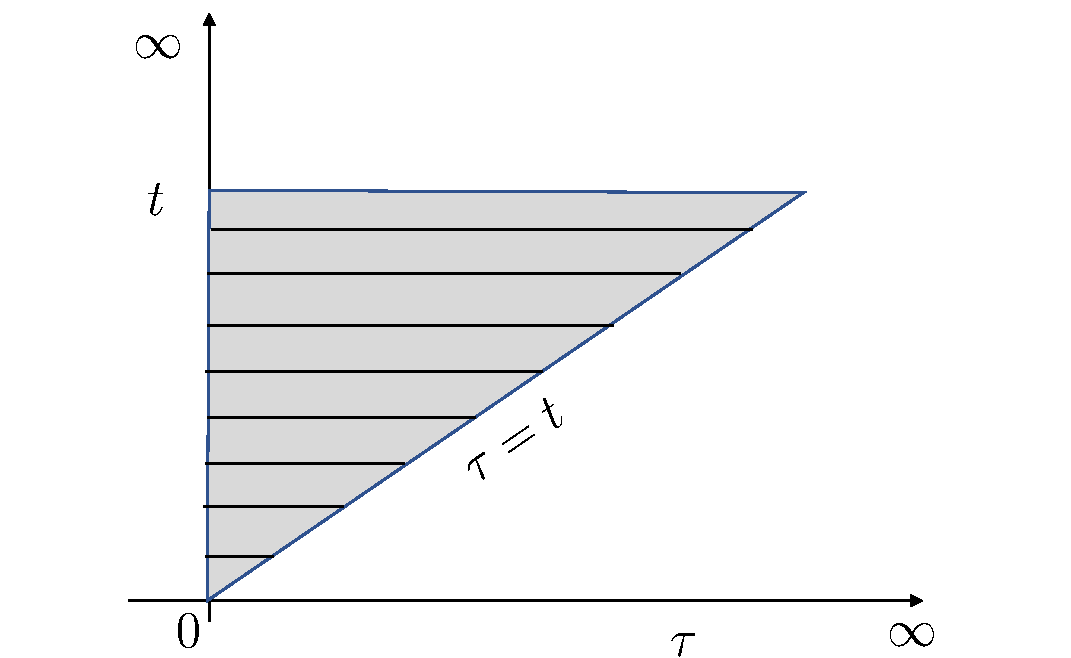
\includegraphics{figures/chap4_order_of_integration}
	\end{center}

	Change the order of integration to get
	\begin{align*}
	\int_{\tau=0}^{\infty} \int_{t=\tau}^{\infty} h(t-\tau)x(\tau)y(t)dt d\tau &= \int_0^{\infty} x(t) \int_t^{\infty} h(\tau - t) y(\tau) d\tau dt\\
	&= \int_0^{\infty} x(t)A^\ast[y](t)dt
	\end{align*}
	\[ \Rightarrow \Acal^\ast[y] = \int_t^{\infty}h(\tau - t)y(\tau)d\tau \]
\end{frame}

%----------------------------------
\begin{frame}\frametitle{Adjoint Operator, Example}
	\begin{example}[linear ode's]
		\[ \dot{x} = Fx \quad ; \quad x(0) = x_0 \]
		
		\vfill
		
		The solution is $x(t) = e^{Ft}x_0$
		
		\vfill
		
		Let $\Acal[x_0](t) = e^{Ft}x_0$, then
		\[ \Acal:\mathbb{R}^n \to L_{2[0,T]} \]
		
		\vfill 
		
		What is $\Acal^\ast$?
	\end{example}
\end{frame}

%----------------------------------
\begin{frame}\frametitle{Adjoint Operator, Example, linear ODE, cont.}
	Let $x \in \mathbb{R}^n$ and let $y \in L_2[0,T]$ then by definition,
		\begin{align*}
			\iprod{\Acal[x_0],y }_{L_2[0,T]} &= \iprod{x_0, \Acal^\ast y }_{\mathbb{R}^n} \\
			\iff \int_0^T x_0^\top(e^{Ft})^\top y(t)dt &= x_0^\top \Acal^\ast y \\
			\iff x_0^\top \int_0^T e^{F^\top t}y(t) dt &= x_0^\top \Acal^\ast y \\
			\Rightarrow \fbox{ $\Acal^\ast[y] = \displaystyle \int_0^Te^{F^\top t}y(t)dt $ }\\
		\end{align*}
\end{frame}


%%%%%%%%%%%%%%%%%%%%%%%%%%%%%%%%%%%%%%%%%%%%%%%%%%%%%%%%%%%%%%%%%
\section{Fundamental Subspaces}
\frame{\sectionpage}

%----------------------------------
\begin{frame}\frametitle{Fundamental Subspaces}
	Let $\Acal: \mathcal{H}_1 \to \mathcal{H}_2$ where $\mathcal{H}_1$ and $\mathcal{H}_2$ are Hilbert spaces. \\
	Then $\Acal^\ast:\mathcal{H}_2 \to \mathcal{H}_1$ and we have the following picture:\\
	\begin{center}
		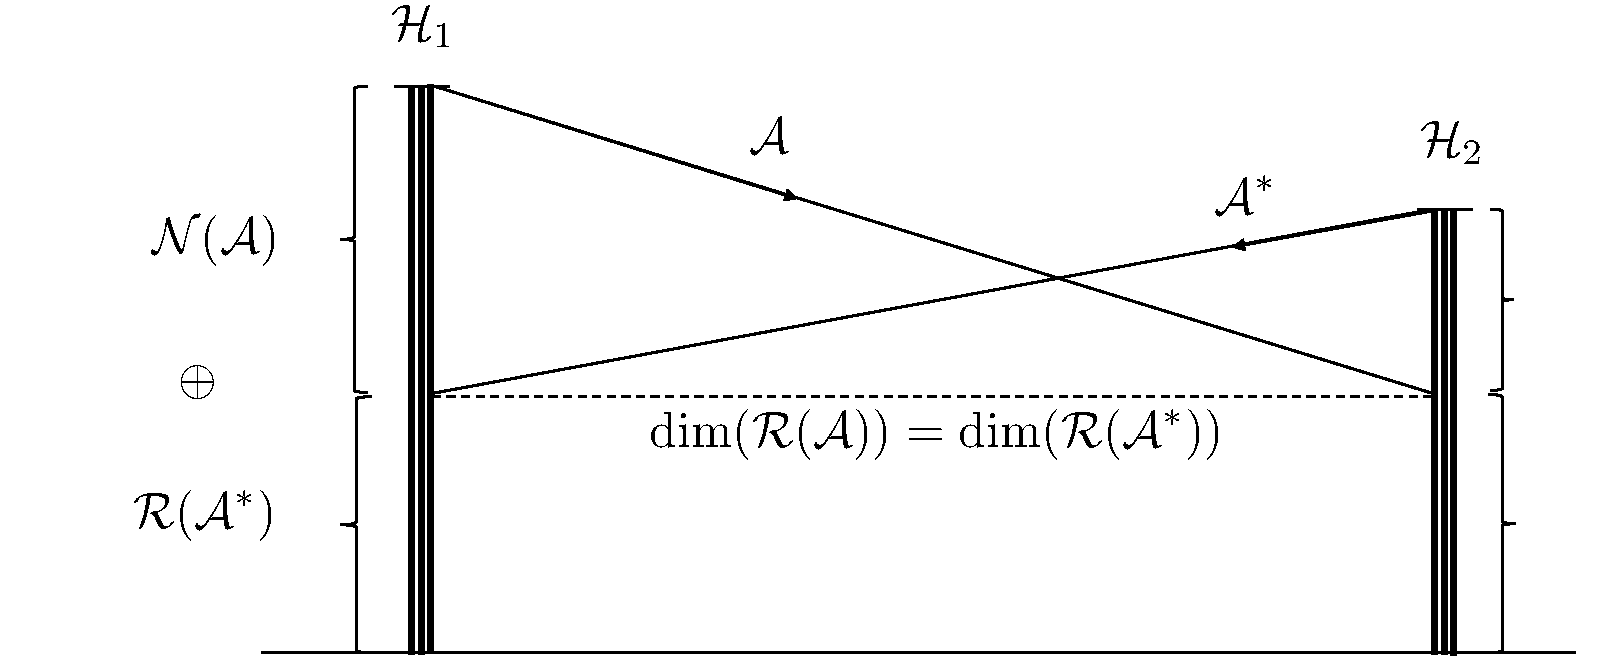
\includegraphics[width=4in]{figures/chap4_fundamental_subspaces}\\
	\end{center}
\end{frame}

%----------------------------------
\begin{frame}\frametitle{Fundamental Subspaces, cont.}
	\begin{lemma}
		\begin{enumerate}
		\item $\mathcal{H}_1 = \mathcal{N}(\Acal) \oplus \mathcal{R}(\Acal^\ast)$
		\item $\mathcal{H}_2 = \mathcal{N}(\Acal^\ast) \oplus \mathcal{R}(\Acal)$
		\item $\dim(\mathcal{H}_1) = \dim(\mathcal{N}(\Acal)) + \dim(\mathcal{R}(\Acal^\ast))$
		\item $\dim(\mathcal{H}_2) = \dim(\mathcal{N}(\Acal^\ast)) + \dim(\mathcal{R}(\Acal))$\\
		\item $\dim(\mathcal{R}(\Acal)) = \dim(\mathcal{R}(\Acal^\ast))$
		\end{enumerate}
	\end{lemma}
	
	Proofs to follow.
	
\end{frame}

%----------------------------------
\begin{frame}\frametitle{Fundamental Subspaces for Matrices}
	For matrices, the picture looks as follows:
	\[ A:\mathbb{C}^n \to \mathbb{C}^m \]
	\[ A^\ast = A^H: \mathbb{C}^m \to \mathbb{C}^n\]
	\begin{center}
		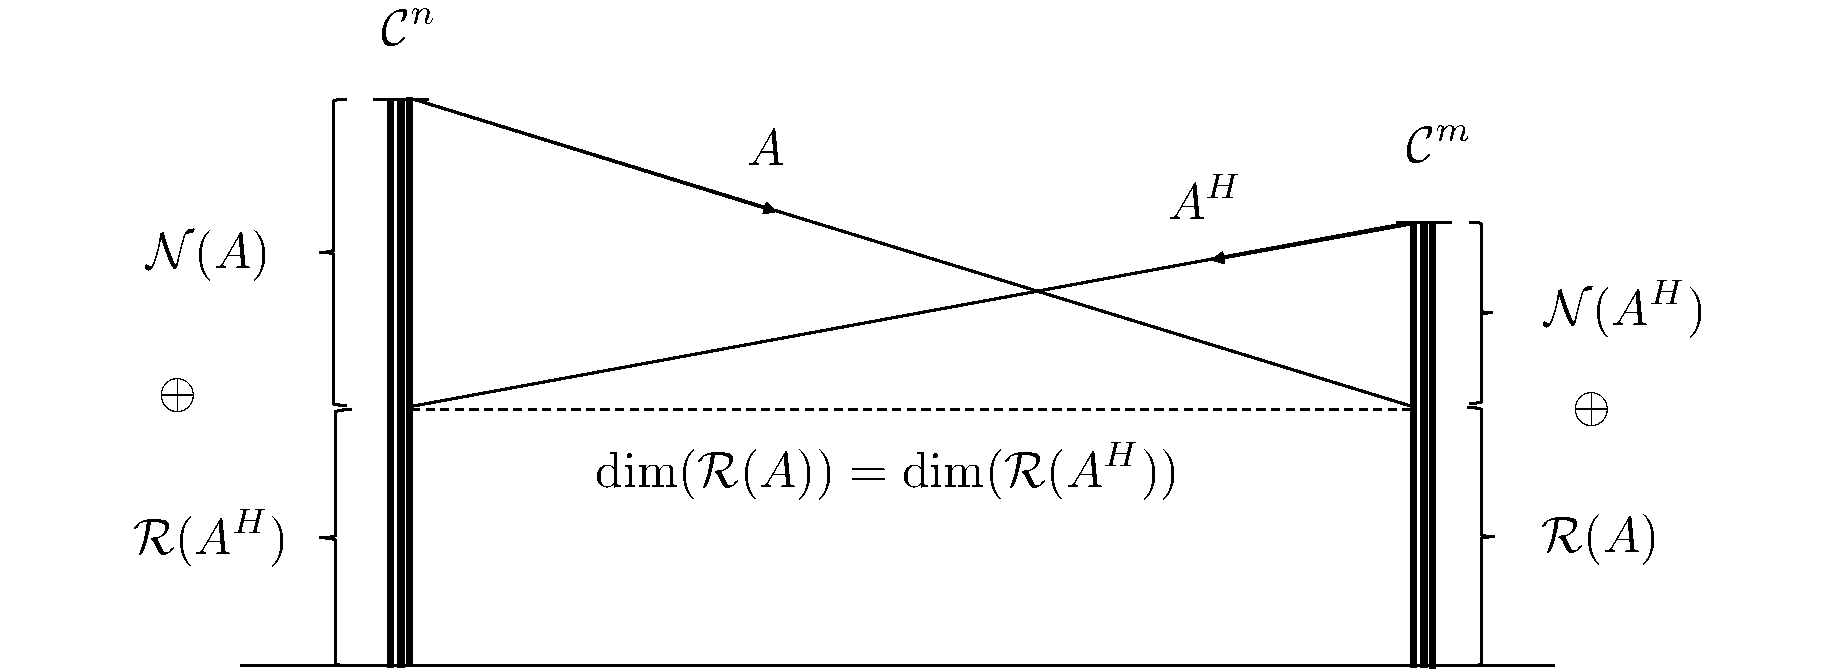
\includegraphics[width=4in]{figures/chap4_fundamental_subspace_matrices}
	\end{center}
	\[\dim(\mathcal{R}(A^H)) = \dim(\mathcal{R}(A))\]
\end{frame}

%----------------------------------
\begin{frame}\frametitle{Fundamental Subspaces, cont}
	\begin{theorem}[Moon Theorem 4.5]	
		Let $\Acal: \mathcal{H}_1 \to \mathcal{H}_2$ be bounded and let $\mathcal{H}_1$ and $\mathcal{H}_2$ be Hilbert spaces and let $\mathcal{R}(\Acal)$ and $\mathcal{R}(\Acal^\ast)$ be closed, then
		\begin{enumerate}
		\item $\left[ \mathcal{R}(\Acal) \right]^{\perp} = \mathcal{N}(\Acal^\ast) $
		\item $\left[ \mathcal{R}(\Acal^\ast) \right]^{\perp} = \mathcal{N}(\Acal) $
		\end{enumerate}	
	\end{theorem}
\end{frame}

%----------------------------------
\begin{frame}\frametitle{Theorem 4.5, Proof}
	\underline{(1):}  To show that $\left[ \mathcal{R}(\Acal) \right]^{\perp} = \mathcal{N}(\Acal^\ast)$ we need to show that $\mathcal{N}(\Acal^{\perp}) \subseteq \left[\mathcal{R}(\Acal)\right]^{\perp}$ and $\left[ \mathcal{R}(\Acal)\right]^{\perp} \subseteq \mathcal{N}(\Acal^\ast)$.
	
	\vfill
	
	\underline{We first show that $\mathcal{N}(\Acal^\ast) \subseteq \left[\mathcal{R}(\Acal)\right]^{\perp}$:}
	
	\vfill
	
	Select any $y \in \mathcal{N}(\Acal^\ast)$ and any $\hat{y} \in \mathcal{R}(\Acal)$.  
	Then $\exists \hat{x} \in \mathcal{H}_1$ such that $\hat{y} = \Acal\hat{x}$.  Therefore
	\begin{align*}
		\iprod{\hat{y}, y } &= \iprod{\Acal\hat{x},y } \\
			&= \iprod{\hat{x}, \Acal^\ast y }\\
			&= \iprod{\hat{x}, 0 } = 0 \\
		\Rightarrow &\quad y \in \left[ \mathcal{R}(\Acal) \right]^{\perp} \\
		\Rightarrow &\quad \mathcal{N}(\Acal^\ast) \subseteq \left[\mathcal{R}(\Acal)\right]^{\perp}
	\end{align*}
\end{frame}

%----------------------------------
\begin{frame}\frametitle{Theorem 4.5, Proof, cont.}

	\underline{We first show that $\left[ \mathcal{R}(\Acal)\right]^{\perp} \subseteq \mathcal{N}(\Acal^\ast)$:}
	
	\vfill
	
	Select any $y \in \left[ \mathcal{R}(\Acal)\right]^{\perp}$.  For every $\hat{x} \in \mathcal{H}_1$ we have $\hat{y} = \Acal\hat{x}\in\Rcal(\Acal)$, and therefore
	\[ \iprod{\hat{y},y }= \iprod{\Acal\hat{x},y } = 0 \]
	By definition of the adjoint, we therefore have that
	\[ \iprod{\hat{x}, \Acal^\ast y } = 0 \]
	Since this is true for every $\hat{x} \in \mathcal{H}_1$ it must be that $\Acal^\ast y = 0$.  Therefore
	\[ y \in \mathcal{N}(\Acal^\ast), \]	
	which implies that
	\[\left[ \mathcal{R}(\Acal)\right]^{\perp} \subseteq \mathcal{N}(\Acal^\ast).\]
	
	\vfill
	
	Item (2) is shown similarly.
\end{frame}

%----------------------------------
\begin{frame}\frametitle{Fundamental Subspaces, cont}
	Theorem 2.10 states that if $\mathcal{H}$ is a Hilbert space and if $\mathbb{V}$ a closed subspace in $\mathcal{H}$ then
	\[ \mathcal{H} = \mathbb{V} \oplus \mathbb{V}^{\perp} \]
	
	\vfill
	
	Therefore Theorem 4.5 implies that
	\begin{align*}
		\mathcal{H}_1 &= \mathcal{R}(\Acal^\ast) \oplus \mathcal{N}(\Acal) \\
		\mathcal{H}_2 &= \mathcal{R}(\Acal) \oplus \mathcal{N}(\Acal^\ast)
	\end{align*}
	
	\vfill
	
	Which also implies that
	\begin{align*}
		\dim(\mathcal{H}_1) &= \dim(\mathcal{R}(\Acal^\ast)) + \dim(\mathcal{N}(\Acal)) \\
		\dim(\mathcal{H}_2) &= \dim(\mathcal{R}(\Acal)) + \dim(\mathcal{N}(\Acal^\ast))
	\end{align*}
\end{frame}

%----------------------------------
\begin{frame}\frametitle{Fundamental Subspaces, cont}
	\begin{columns}
		\begin{column}{0.5\textwidth}
				\begin{lemma}
					\begin{itemize}
						\item $\mathcal{R}(\Acal) = \mathcal{R}(\Acal\Acal^\ast)$
						\item $\mathcal{R}(\Acal^\ast) = \mathcal{R}(\Acal^\ast\Acal)$
					\end{itemize}
				\end{lemma}
		\end{column}
		\begin{column}{0.5\textwidth}
			\begin{center}
				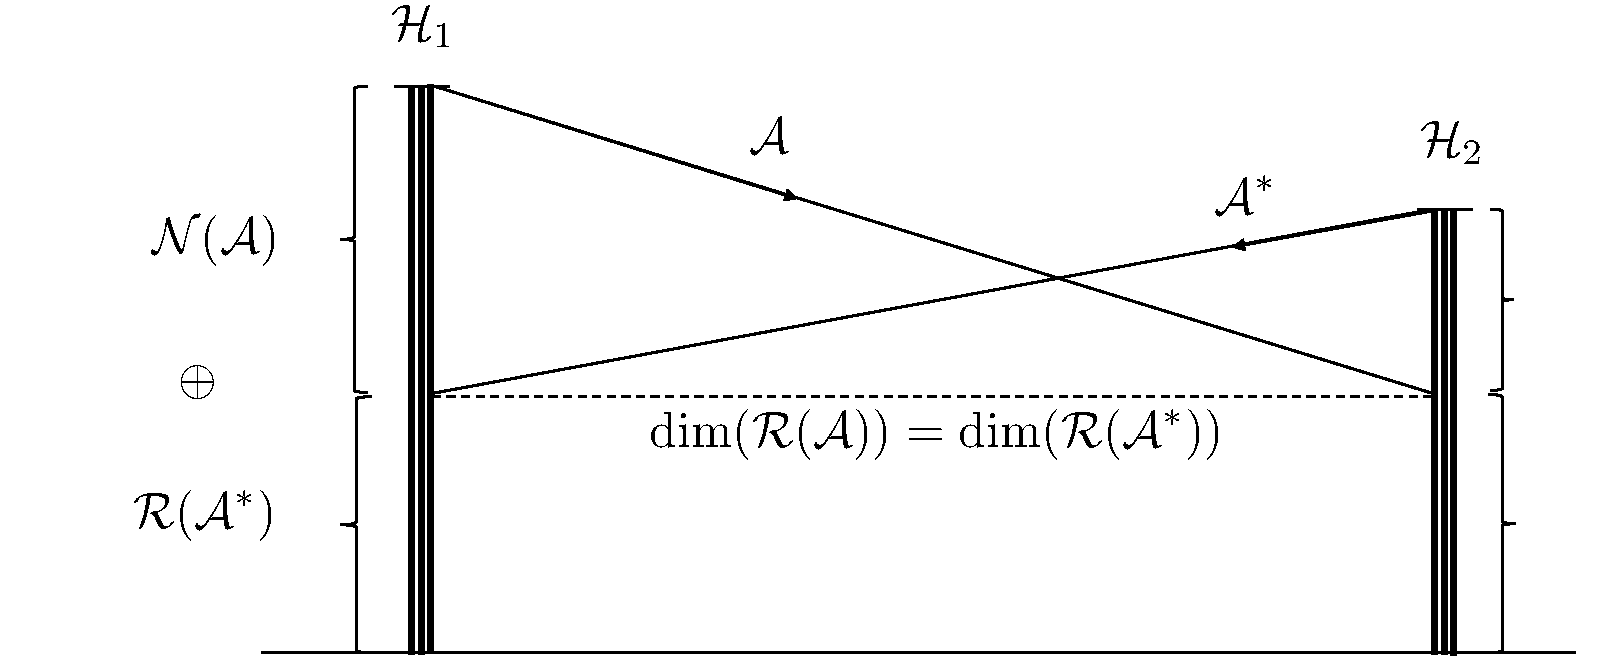
\includegraphics[width=\textwidth]{figures/chap4_fundamental_subspaces}
			\end{center}	
		\end{column}
	\end{columns}

	\begin{proofstart}
		We will prove (1) by showing that:
		\begin{description}
		\item[(a)] 	$\mathcal{R}(\Acal) \subseteq \mathcal{R}(\Acal\Acal^\ast)$
		\item[(b)]  $\mathcal{R}(\Acal\Acal^\ast) \subseteq \mathcal{R}(\Acal)$
		\end{description}
	\end{proofstart}
	
\end{frame}

%----------------------------------
\begin{frame}\frametitle{Fundamental Subspaces, cont}
	\begin{proof}[Proof (cont.)]
		\noindent (a) Let $y \in \mathcal{R}(\Acal) \Rightarrow \exists x \in \mathcal{H}_1 $ such that $ y = \Acal x$

		Since $\mathcal{H}_1 = \mathcal{R}(\Acal^\ast) \oplus \mathcal{N}(\Acal), \quad x  = x_n + x_r$ where
		\[ x_n \in \mathcal{N}(\Acal) \text{ and } x_r \in \mathcal{R}(\Acal^\ast) \]
		\[ \Rightarrow \exists \hat{y} \in \mathcal{H}_2 \text{ such that } x_r = \Acal^\ast\hat{y}\]
		so
		\[ y = \Acal x = \Acal(x_n + x_r) = \Acal\Acal^\ast\hat{y} \]
		\[ \Rightarrow y \in \mathcal{R}(\Acal\Acal^\ast) \]	 
		
		\noindent (b) let $y \in \mathcal{R}(\Acal\Acal^\ast) \Rightarrow \exists \hat{y} \in \mathcal{H}_2 $ such that
		\[ y = \Acal\Acal^\ast\hat{y} \Rightarrow y = \Acal\hat{x} \text{ where } \hat{x} \in \mathcal{H}_1 \]
		\[ \Rightarrow y \in \mathcal{R}(\Acal). \]	
	\end{proof}
	
\end{frame}

%----------------------------------
\begin{frame}\frametitle{Fundamental Subspaces, cont}
	\begin{theorem}
		\[ 
		\dim(\Rcal(\Acal)) = \dim(\Rcal(\Acal^\ast)) 
		\]
	\end{theorem}
	
	\begin{proofstart}
		We need to show that
		\begin{description}
			\item[(a)] $ \dim(\Rcal(\Acal)) \leq \dim(\Rcal(\Acal^\ast)) $
			\item[(b)]\ $ \dim(\Rcal(\Acal^\ast)) \leq \dim(\Rcal(\Acal)) $
		\end{description}
	\end{proofstart}
\end{frame}

%----------------------------------
\begin{frame}\frametitle{Fundamental Subspaces, cont}
	\begin{proofstart}[Proof (cont.)]
		(a) Let $P = \{ p_1, p_2, \ldots \}$ be a Hamel basis for $\mathcal{R}(\Acal)$ so $\dim(\mathcal{R}(\Acal)) = \mathit{cardinality}$ of $P$.
		\[ p_i \in \mathcal{R}(\Acal) \Rightarrow \exists \hat{q}_i \in \mathcal{H}_1 \text{ such that } p_i = \Acal\hat{q}_i \]
		\[ \mathcal{H}_1 = \mathcal{R}(\Acal^\ast) \oplus \mathcal{N}(\Acal) \Rightarrow \hat{q}_i = q_{i,n} + q_i \]
		\[ \text{ where } q_{i,n} \in \mathcal{N}(\Acal) \text{ and } q_i \in \mathcal{R}(\Acal^\ast) \]
		\[ \Rightarrow p_i = \Acal q_i,\] let
		\[ Q = \{ q_1, q_2, \ldots \} \] we will show that $Q$ is linearly independent $\Rightarrow $ any Hamel basis of $\mathcal{R}(A^\ast)$ contains $Q \Rightarrow \dim(\mathcal{R}(A^\ast)) \geq \dim(\mathcal{R}(A))$,


	\end{proofstart}
\end{frame}

%----------------------------------
\begin{frame}\frametitle{Fundamental Subspaces, cont}
	\begin{proof}[Proof (cont.)]
		$P$ is a Hamel basis $\Rightarrow$ all finite subsets of $P$ are linearly independent, i.e.
		\[ \sum_{i \in I} c_ip_i = 0 \iff c_i = 0, i \in I \]
		where $I$ is a finite index set.  But,
		\[ \sum_I c_ip_i = 0 \iff \sum_I c_i\Acal q_i = 0 \iff \Acal(\sum_I c_iq_i) = 0 \]
		but
		$ \sum_I c_i q_i \in \mathcal{R}(\Acal^\ast) \perp \mathcal{N}(\Acal) $\\
		so
		\[ \iff \sum_I c_i q_i = 0 \iff c_i = 0, i \in I \]
		\[ \Rightarrow Q \text{ is linearly independent } \]
		
		(b) Substitute $\Acal$ for $\Acal^\ast$ and $\Acal^\ast$ for $\Acal$ is above argument.

	\end{proof}
	
\end{frame}


%----------------------------------
\begin{frame}\frametitle{Solution of Operator Equations}
	We turn to solutions to the linear operator equation
	\[ \Acal x = y \]
	where $\Acal:\mathcal{H}_1 \to \mathcal{H}_2 $ is bounded, $\mathcal{H}_1$ and $\mathcal{H}_2$ are Hilbert and $\mathcal{R}(\Acal)$ is closed.
	
		\begin{multicols}{2}
			\begin{description}
			\item[Fact 1.]	$\Acal x = y$ has a solution $\iff y \in \mathcal{R}(\Acal) $
			\item[Fact 2.] $\Acal x = y$ has a solution $\iff y \perp \mathcal{N}(\Acal^\ast)$
			\end{description}
 
			\columnbreak

			\begin{center}
				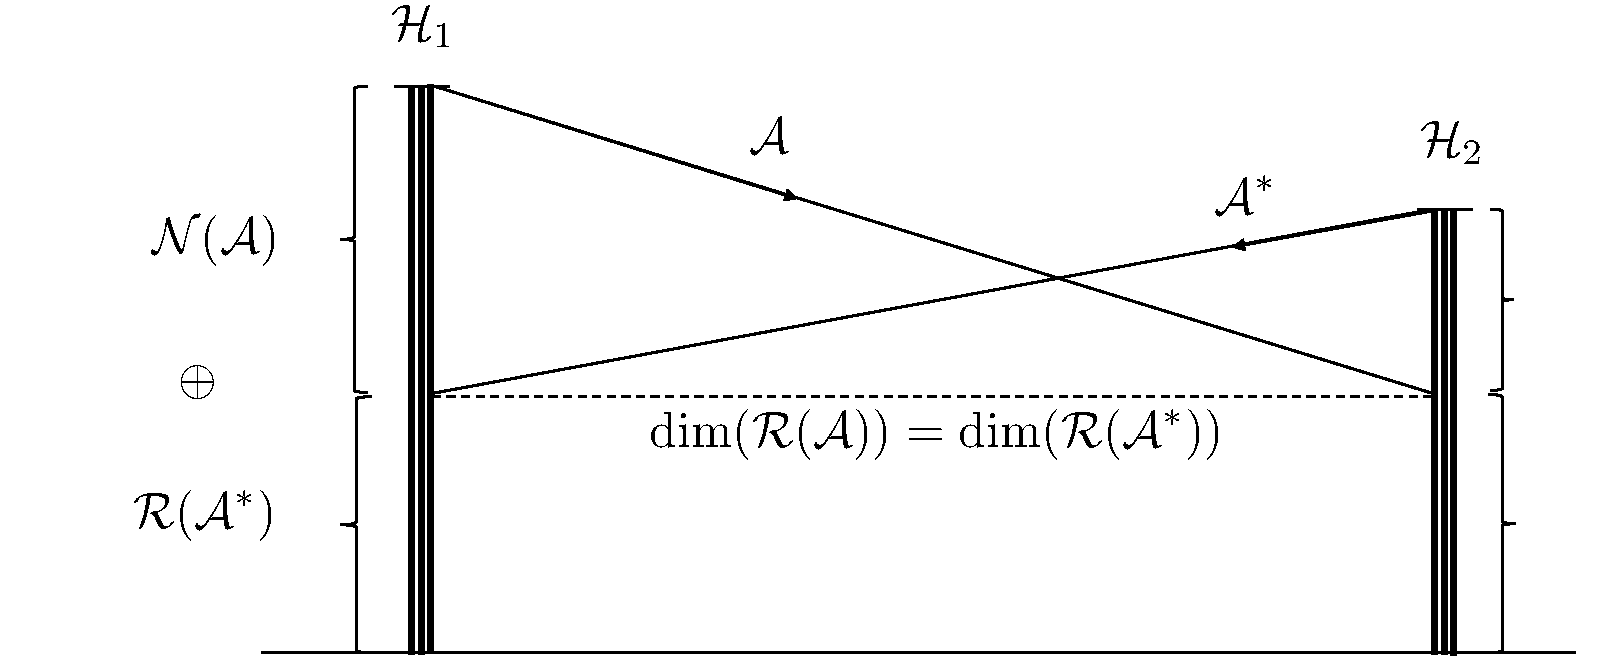
\includegraphics[width=2in]{figures/chap4_fundamental_subspaces}
			\end{center}	
		\end{multicols}

\end{frame}

%----------------------------------
\begin{frame}\frametitle{Solution of Operator Equations}
	\begin{description}
		\item[Fact 3.] If $\Acal x = y$ has a solution then it is unique $\iff \mathcal{N}(\Acal) = \{0\}$
		\item[Fact 4.]  If $\mathcal{N}(\Acal) \neq \{0\}$ and $y \in \mathcal{R}(\Acal)$ then $\Acal x = y$ has an infinite number of solutions.
		\item[Fact 5].  $\Acal^{-1}$ exists $\Rightarrow \mathcal{N}(\Acal) = \{0\}$ (otherwise can't get back to all of $\mathcal{H}$.
	\end{description}
 
	\begin{center}
		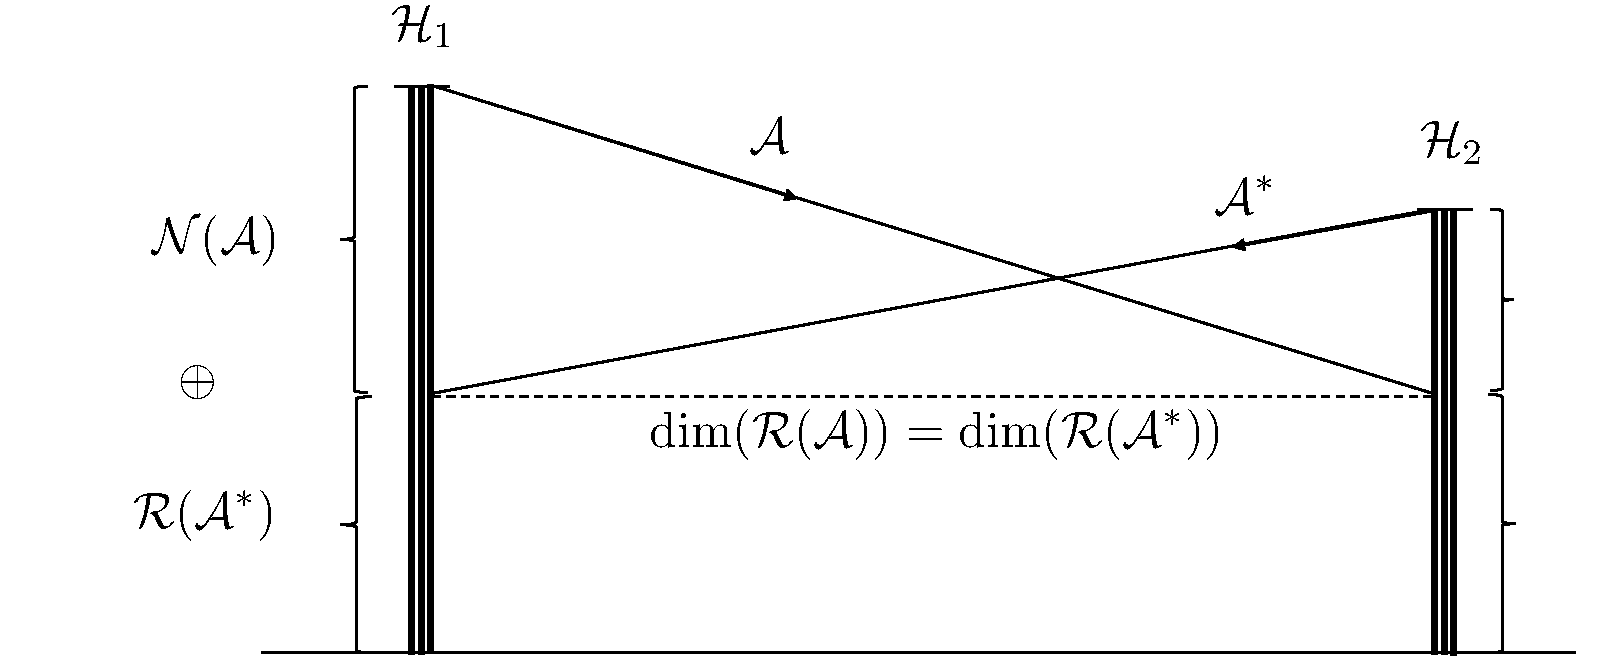
\includegraphics[width=4in]{figures/chap4_fundamental_subspaces}
	\end{center}	
\end{frame}


%----------------------------------
\begin{frame}\frametitle{Matrix Rank}
	\begin{definition}[Row Rank] 
		The \underline{row rank} of $A\in\mathbb{C}^{m\times n}$ is the number of linearly independent rows.
	\end{definition}
	\begin{definition}[Column Rank]
		The \underline{column rank} of $A\in\mathbb{C}^{m\times n}$ is the number of linearly independent columns.
	\end{definition}

	\begin{itemize}
		\item Since $\mathcal{R}(A) = span\{\text{columns of } A\}$ we have that $\dim(\mathcal{R}(A)) = \text{ column rank }$
		\item Since $\mathcal{R}(A^H) = span\{\text{rows of } A\}$ we have that $\dim(\mathcal{R}(A^\ast)) = \text{ row rank } $
		\item Therefore $\dim(\mathcal{R}(A)) = \dim(\mathcal{R}(A^H))$ implies that $\text{ column rank } = \text{ row rank }$
	\end{itemize}
\end{frame}

%----------------------------------
\begin{frame}\frametitle{Matrix Rank}
	\begin{definition}
		The rank of $A$ is the number of linearly independent rows or columns.
	\end{definition}
	
	\begin{lemma}
		\[ rank(A) = rank(A^H) \]
	\end{lemma}

	\begin{definition}
		$A: \mathbb{C}^n\to \mathbb{C}^m $ is full rank if $rank(A) = \min(n,m)$
	\end{definition}
	
\end{frame}

%----------------------------------
\begin{frame}\frametitle{Sylvester's Inequality}
	\begin{lemma}[Sylvester's Inequality]
		Let $A \in \mathbb{C}^{q\times n}$ and $B \in \mathbb{C}^{n \times p}$ then 
		\[
			rank(A) + rank(B) - n \leq rank(AB) \leq \min(rank(A),rank(B)).
		\]
	\end{lemma}
	
	\vfill

	\begin{example}
	Let $x \in \mathbb{R}^m$ and $y \in \mathbb{R}^n$ then
	\[ rank(xy^\top) = 1 \]
	
	\end{example}
\end{frame}

%%%%%%%%%%%%%%%%%%%%%%%%%%%%%%%%%%%%%%%%%%%%%%%%%%%%%%%%%%%%%%%%%
\section{Matrix Inverses}
\frame{\sectionpage}

%----------------------------------
\begin{frame}\frametitle{Matrix Inverses}
	\begin{definition}
		$A \in \mathbb{C}^{m\times n}$ has a \underline{left} inverse if $\exists B \in \mathbb{C}^{n \times m}$ such that
		\[ \underset{n \times m}{B} \quad \underset{m \times n}{A} = \underset{n \times n}{I}\]
	\end{definition}
	\begin{definition}
		$A \in \mathbb{C}^{m \times n}$ has a \underline{right} inverse if $\exists D \in \mathbb{C}^{n \times m}$ such that 
		\[ \underset{m \times n}{A} \quad \underset{n \times m}{C} = \underset{m \times m}{I} \]
	\end{definition}
\end{frame}

%----------------------------------
\begin{frame}\frametitle{Matrix Inverses, cont}
	
	\begin{example}
		The matrix
		\[ A = \begin{pmatrix} 2 & 0 & 0\\ 0 & 7 & 0 \end{pmatrix}. \]
		has an infinite number of right inverses, namely
		\[ C = \begin{pmatrix} \frac{1}{2} & 0\\ 0 & \frac{1}{7}\\ c_1 & c_2 \end{pmatrix} 
			\qquad \forall c_1,c_2 \in \mathbb{R} \]
		since 
		\[
		AC = \begin{pmatrix} 1 & 0\\ 0 & 1 \end{pmatrix}.
		\]
	\end{example}
	
\end{frame}


%----------------------------------
\begin{frame}\frametitle{Matrix Inverses, cont}
	\begin{itemize} 
	\item 	Suppose $A$ has a left inverse, then 
	\[ Ax = b \iff BAx = Bb \iff x = Bb \]
	\item Suppose $A$ has a right inverse, then let
	\[ x = Cb \Rightarrow Ax = ACb = b\]
	so $x = Cb$ is a solution.
	\end{itemize}
\end{frame}

%----------------------------------
\begin{frame}\frametitle{Left Inverse}
	\begin{columns}
		\begin{column}{0.6\textwidth}
			\begin{itemize}
			\item 	Let $B$ be a left inverse of $A$.  
			\item Then $BA=I:\mathbb{C}^n\to\mathbb{C}^n$.  
			\item Of necessity we must have that $\mathcal{N}(A) = \{0\}$, otherwise there are vectors $x\in\mathcal{N}(\Acal)\subseteq \mathbb{C}^n$ such that $BAx = B0 = 0 \neq x$, i.e., $BA\neq I$.
			\item Therefore $Ax = b$ has \underline{at most} one solution \\(since $b$ may not be in $\mathcal{R}(A)$).
			\end{itemize}
		\end{column}
		\begin{column}{0.5\textwidth}
			\begin{center}
	  			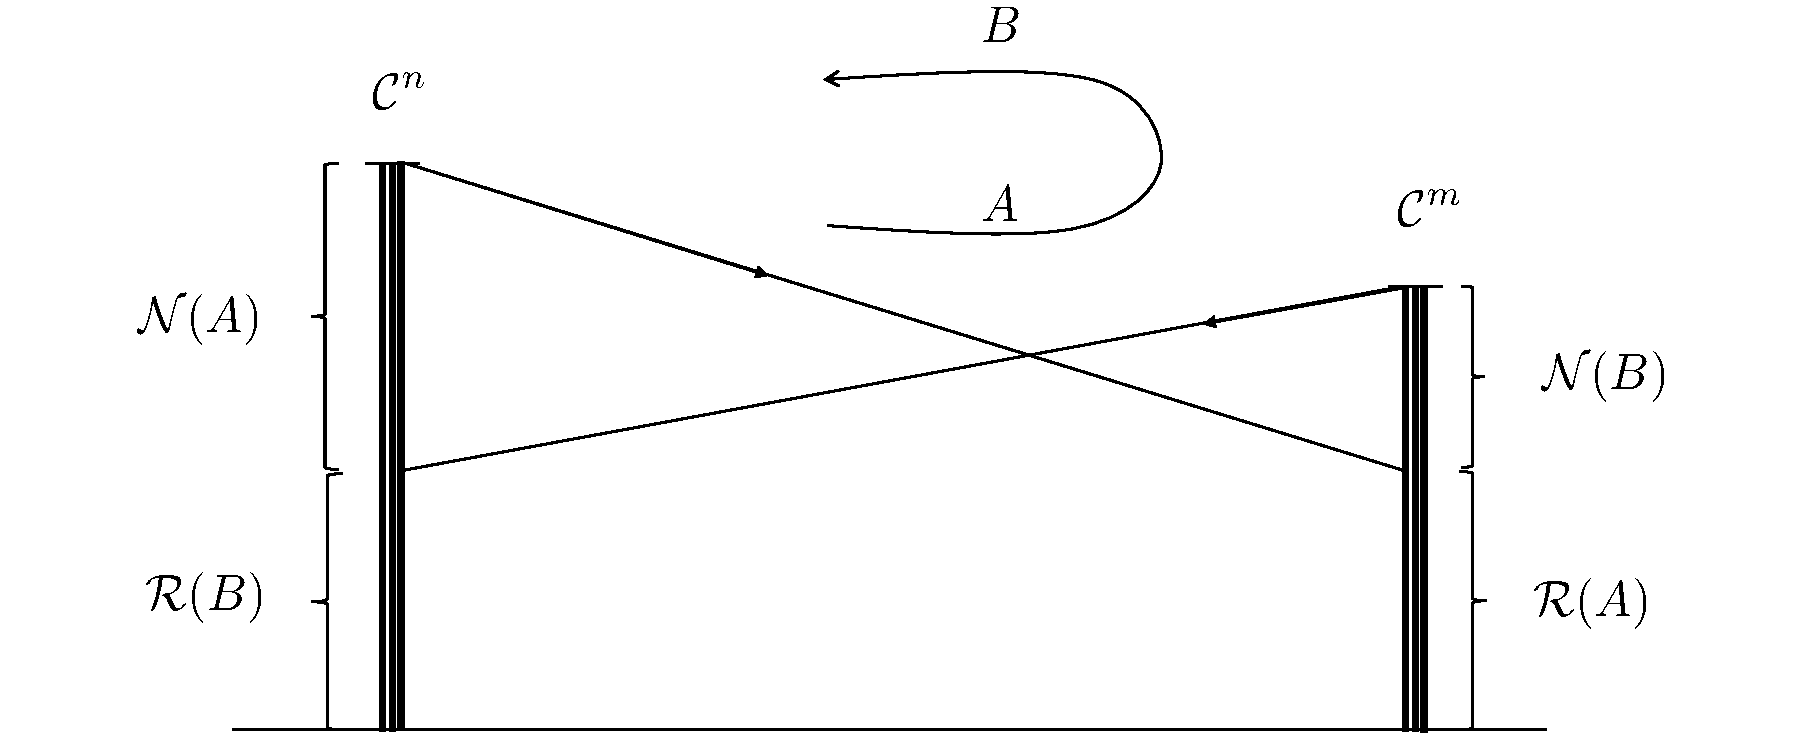
\includegraphics[width=\textwidth]{figures/chap4_left_inverse}	
			\end{center}
			\begin{center}	
	  			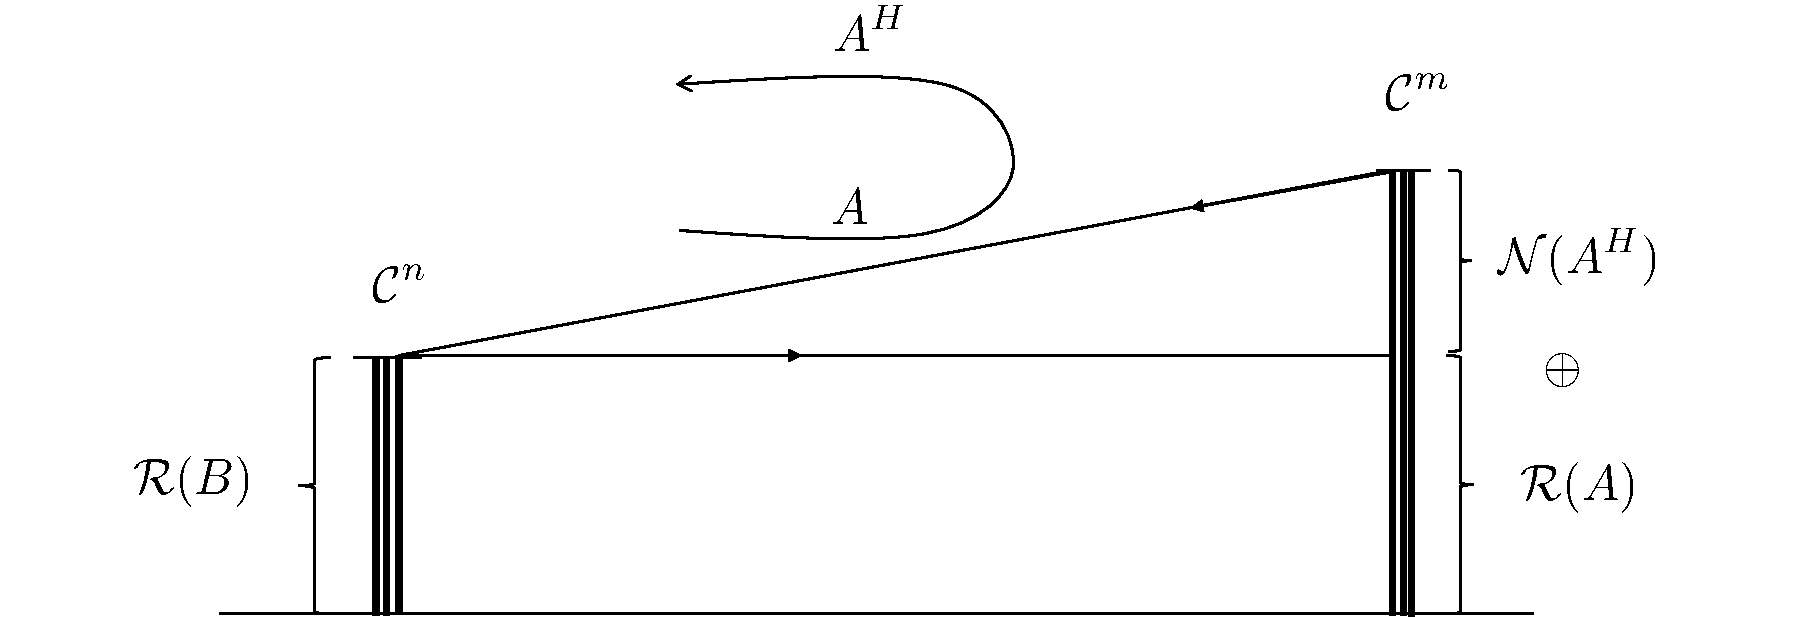
\includegraphics[width=\textwidth]{figures/chap4_left_inverse_full_rank}
			\end{center}
		\end{column}
	\end{columns}
\end{frame}

%----------------------------------
\begin{frame}\frametitle{Right Inverse}
	\begin{columns}
		\begin{column}{0.6\textwidth}
			\begin{itemize}
			\item 	Let $D$ be a right inverse of $A$.  
			\item Then $AD=I:\mathbb{C}^m\to\mathbb{C}^m$.  
			\item Of necessity we must have that $\mathcal{N}(A^H) = \{0\}$, otherwise $D^H A^H = I$ is impossible.
			\item 	$\mathcal{N}(A)$ may be nontrivial therefore if $\hat{x}$ is a solutions so is $\hat{x} + x_n$ where $x_n \in \mathcal{N}(A)$ since $A(\hat{x}+x_n) = A\hat{x} = b$.  Therefore, there is \underline{at least one} solution.
			\end{itemize}
		\end{column}
		\begin{column}{0.5\textwidth}
			\begin{center}
	  			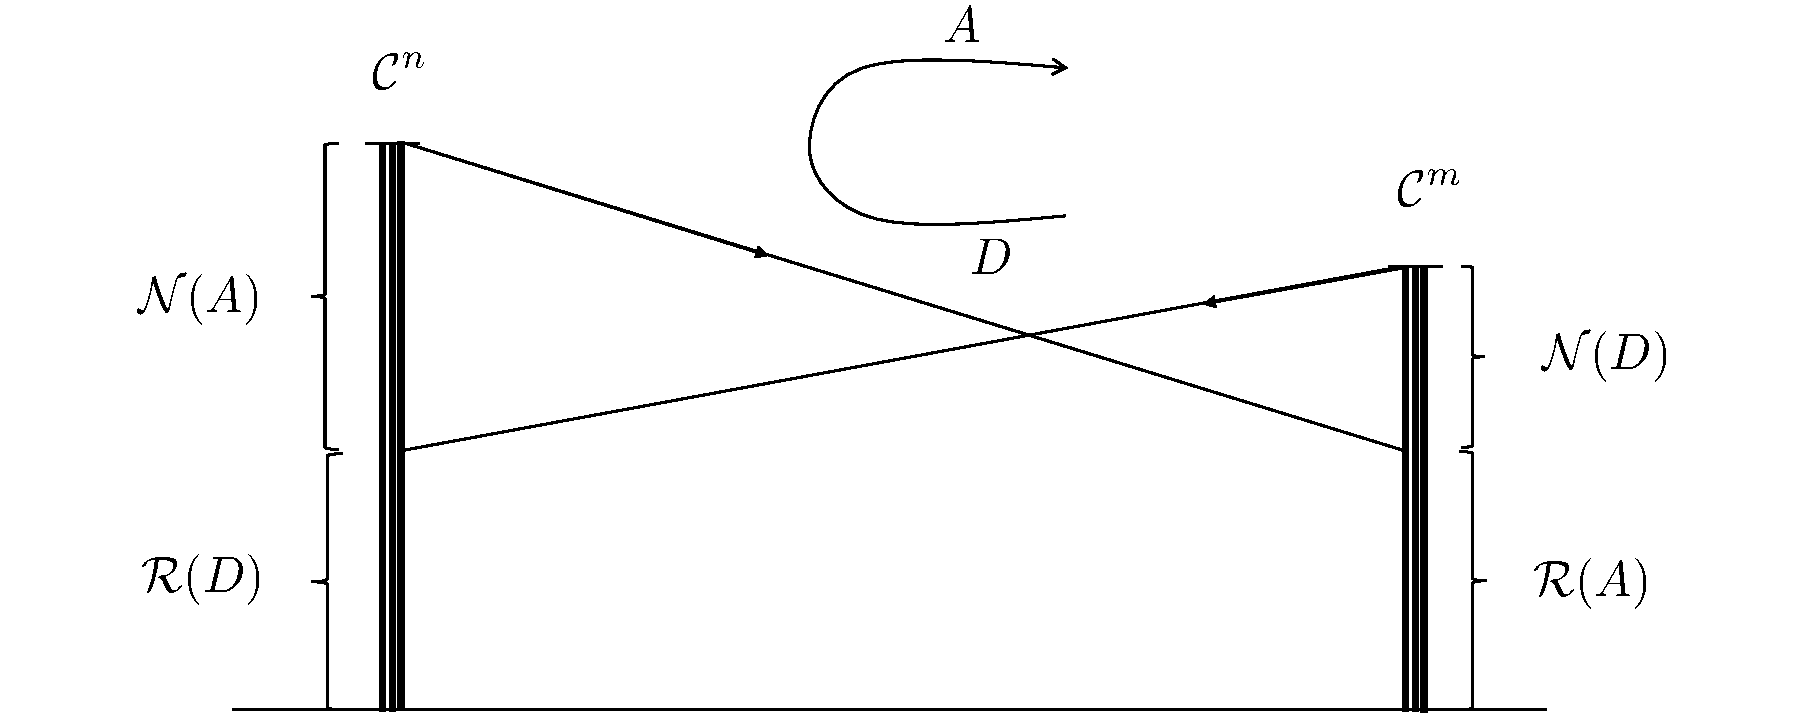
\includegraphics[width=\textwidth]{figures/chap4_right_inverse}	
			\end{center}
			\begin{center}	
	  			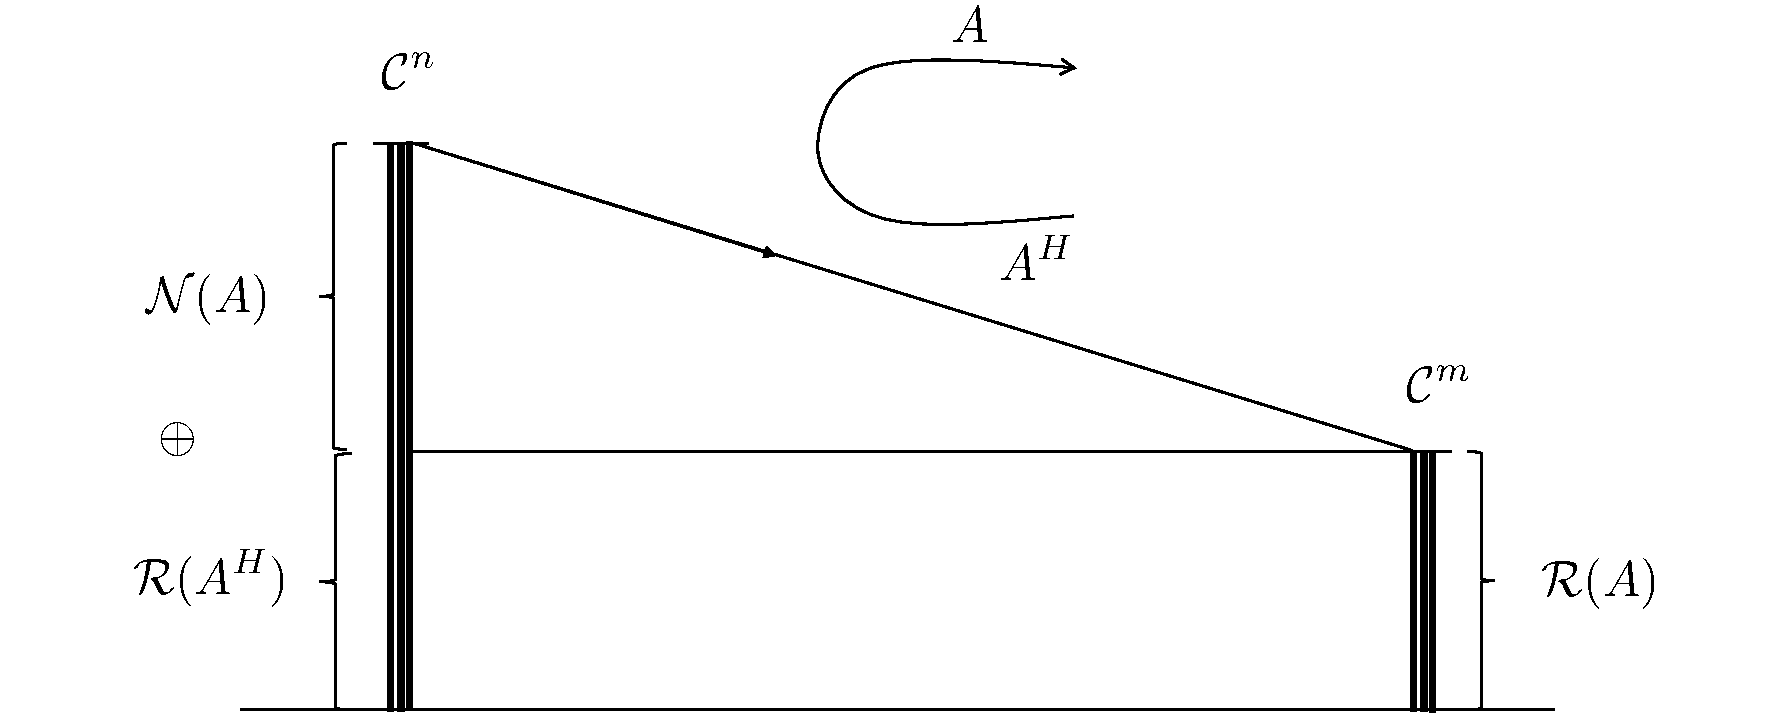
\includegraphics[width=\textwidth]{figures/chap4_right_inverse_full_rank}
			\end{center}
		\end{column}
	\end{columns}
\end{frame}

%----------------------------------
\begin{frame}\frametitle{Right and Left Inverses}
	\begin{lemma}
		\begin{enumerate}
		\item If $A$ has a left inverse then $Ax = b$ has at most one solution.
		\item If $A$ has a right inverse then $Ax = b$ has at least one solution.
		\end{enumerate}
	\end{lemma}
\end{frame}

%----------------------------------
\begin{frame}\frametitle{Regular Inverse}
	If $A \in \mathbb{C}^{n \times n}$ when the following statements are equivalent:
	\begin{enumerate}
  		\item $A^{-1}$ exists
  		\item $\mathcal{N}(A) = \{0\}$ and $\mathcal{N}(A^H)=\{0\}$.
  		\item $rank(A) = n$
  		\item $det(A) \neq 0$
  		\item (right inverse of $A$) = (left inverse of $A$) = $A^{-1}$
  		\item there are no zero eigenvalues of $A$
  		\item $A^HA$ is positive definite
  		\item $A$ is nonsingular
		\end{enumerate}
\end{frame}

%----------------------------------
\begin{frame}\frametitle{Regular Inverse, cont.}
	If $A^{-1}$ exists then 
	\[
	\boxed{A^{-1} = \frac{adj(A)}{det(A)}}
	\]
	where $adj(A)$ is the adjugate of $A$ where $adj(A) = [B_{ij}]^\top$ and $B_{ij} = (-1)^{i+j}det(M_{ij})$ and $M_{ij}$ is the $(i,j)^{th}$ minor of $A$.

	\begin{example}	
		\[ A = 
			\left( 
  			\begin{array}{cc}
    			a & b\\
    			c & d
  			\end{array}
			\right) 
		\]
		\[ adj(A) = 
			\left( 
  			\begin{array}{cc}
    			(-1)^2|d| & (-1)^3|c|\\
    			(-1)^3|b| & (-1)^4|a|
  			\end{array}
			\right)
		= 
			\left(
  			\begin{array}{cc}
    			d & -c\\
    			-b & a
  			\end{array}
			\right)
		\]
		so
			$A^{-1} = \frac{
			\left( \begin{array}{cc}
			d & -c\\
			-b & a
			\end{array}
			\right)
			}
			{det(A)}
			= \frac{
			\left( \begin{array}{cc}
			d & -c\\
			-b & a
			\end{array} \right)
			}
			{ad - cb}$
	\end{example}
\end{frame}

%----------------------------------
\begin{frame}\frametitle{Matrix Rank}
	\begin{lemma}
		Let $A:\mathbb{C}  ^n \to \mathbb{C}^m$ then
		\[ rank(\underset{m\times n}{A}) = rank(\underset{n \times m}{A^H}) = rank(\underset{n\times n}{A^HA}) = rank(\underset{m\times m}{AA^H}) \]
	\end{lemma}
	
	\begin{proof}
		\begin{align*}
		rank(B) &= \text{ \# of linearly independent columns}
				= \dim(\mathcal{R}(B))\\
				&= \text{ \# of linearly independent rows }
				= \dim(\mathcal{R}(B^H)).
		\end{align*}
		Therefore 
		\begin{align*}
		rank(A) &= \dim(\mathcal{R}(A))
				= \dim(\mathcal{R}(A^H)) = rank(A^H)\\
				&= \dim(\mathcal{R}(AA^H)) =rank(AA^H) \text{ Since $\mathcal{R}(A^\ast) = \mathcal{R}(AA^\ast)$} \\
				&= \dim(\mathcal{R}(A^HA)) = rank(A^HA) \text{ Since $\mathcal{R}(A) = \mathcal{R}(A^\ast A)$}
		\end{align*}
	\end{proof}
\end{frame}

%%----------------------------------
%\begin{frame}\frametitle{Left Inverse: Least Squares}
%	\begin{columns}
%		\begin{column}{0.5\textwidth}
%			\begin{itemize}
%			\item 	Consider the solution of $Ax=b$ where $m>n$, i.e., $A$ is tall.
%			\item Assume $A$ is full rank, i.e., $rank(A)=n$.
%			\item Assume $b \in \mathcal{R}(A)$
%			\end{itemize}
%		\end{column}
%		
%		\begin{column}{0.5\textwidth}
%			\begin{center}
%				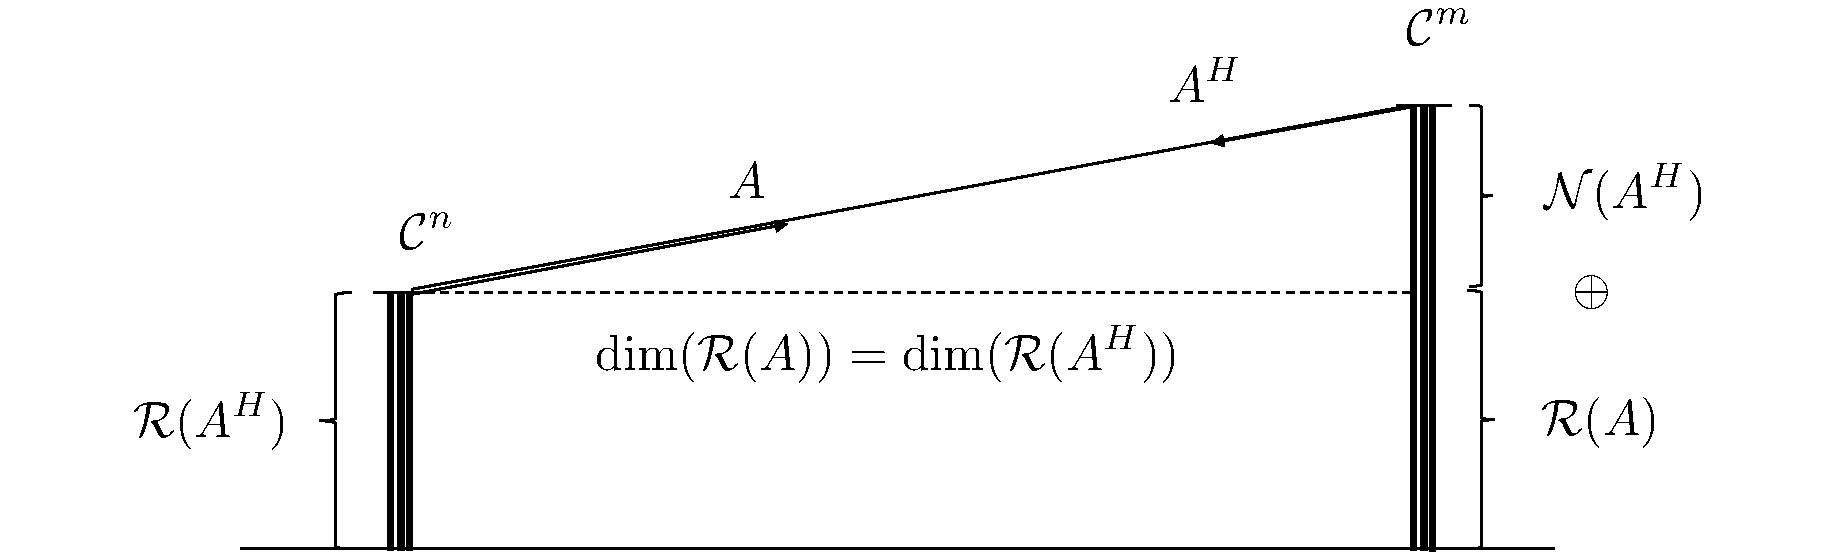
\includegraphics[width=\textwidth]{figures/chap4_least_squares}
%			\end{center}
%		\end{column}
%	\end{columns}
%
%\end{frame}

%----------------------------------
\begin{frame}\frametitle{Left Inverse: Least Squares}
	\begin{itemize}
		\item 	Consider the solution of $Ax=b$ where $m>n$, i.e., $A$ is tall.
		\item Assume $A$ is full rank, i.e., $rank(A)=n$.
		\item Assume $b \in \mathcal{R}(A)$
	\end{itemize}
	\begin{center}
		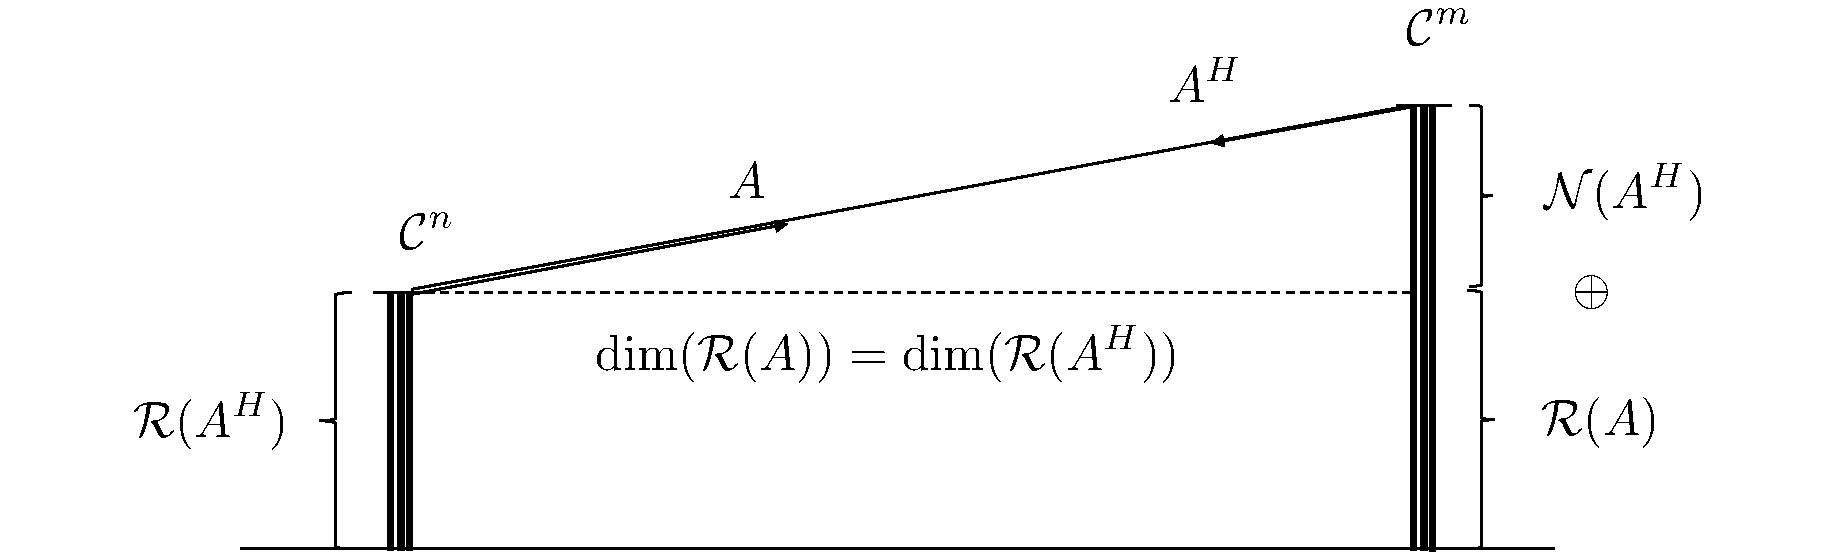
\includegraphics[width=\textwidth]{figures/chap4_least_squares}
	\end{center}
	
	\begin{itemize}
		\item Map $b$ to $\mathcal{R}(A^\ast) :  A^Hb = A^HAx$
		\item Since $rank(A) = n \iff rank(A^HA) = n$ so $(A^HA)^{-1}$ exists
			\[ \Rightarrow \fbox{ $x = (A^HA)^{-1}A^Hb$ } \]
	\end{itemize}
\end{frame}

%----------------------------------
\begin{frame}\frametitle{Left Inverse: Least Squares, cont.}
	What if $b \notin \mathcal{R}(A)$?  This is the least squares problem, e.g.
	\[
	\underbrace{
		\underbrace{
		\begin{pmatrix}
 	   		a_1 & 1\\
  	  		a_2 & 1\\
  	  		\vdots & \vdots \\
   	 		a_n & 1
 	 	\end{pmatrix}
		}_A
		\underbrace{
		\begin{pmatrix}
	  		x_1\\
	  		x_2
		\end{pmatrix}
		}_x
		= \underbrace{
		\begin{pmatrix}
  	  		b_1\\
  	  		\vdots\\
  	  		b_n
  		\end{pmatrix}
  		}_b
		}_{\text{ linear regression }}
	\]

	Since there is no solution, it is reasonable to find $x$ that minimizes $\norm{e}_2$ where
	\[ e = Ax - b \].

\end{frame}

%----------------------------------
\begin{frame}\frametitle{Left Inverse: Least Squares, cont.}
	\begin{itemize}
	\item 	Note that $b = b_r + b_n$ where $b_r \in \mathcal{R}(A)$ and $b_n \in \mathcal{N}(A^H)$ so $e = Ax - b_r - b_n.$
	\item Since $Ax - b_r \in \mathcal{R}(A) \perp \mathcal{N}(A^H)$ the best we can do is make $Ax = b_r \Rightarrow e = b_n$.
	\item Since $b_n \in \mathcal{N}(A^H) $ we have 
		\begin{align*}
			& 0 = A^HAx - A^Hb_r \\
			\Rightarrow & \underbrace{A^HAx}_{\text{projection of $x$ onto $\mathcal{R}(A^H)$}} = A^Hb_r = \underbrace{A^Hb}_{\text{projection of $b$ onto $\mathcal{R}(A^H)$}}
		\end{align*}
	\item Since $rank(A^HA) = rank(A) = n$ we have
		\[\underbrace{x = (A^HA)^{-1}A^Hb}_{\text{least square solution}}\]
	\end{itemize}
\end{frame}

%----------------------------------
\begin{frame}\frametitle{Right Inverse: Min-Norm Solution}
	\begin{itemize}
		\item 	Consider the solution of $Ax=b$ where $m<n$, i.e., $A$ is fat.
		\item Assume $A$ is full rank, i.e., $rank(A)=m$.
	\end{itemize}
	\begin{center}
		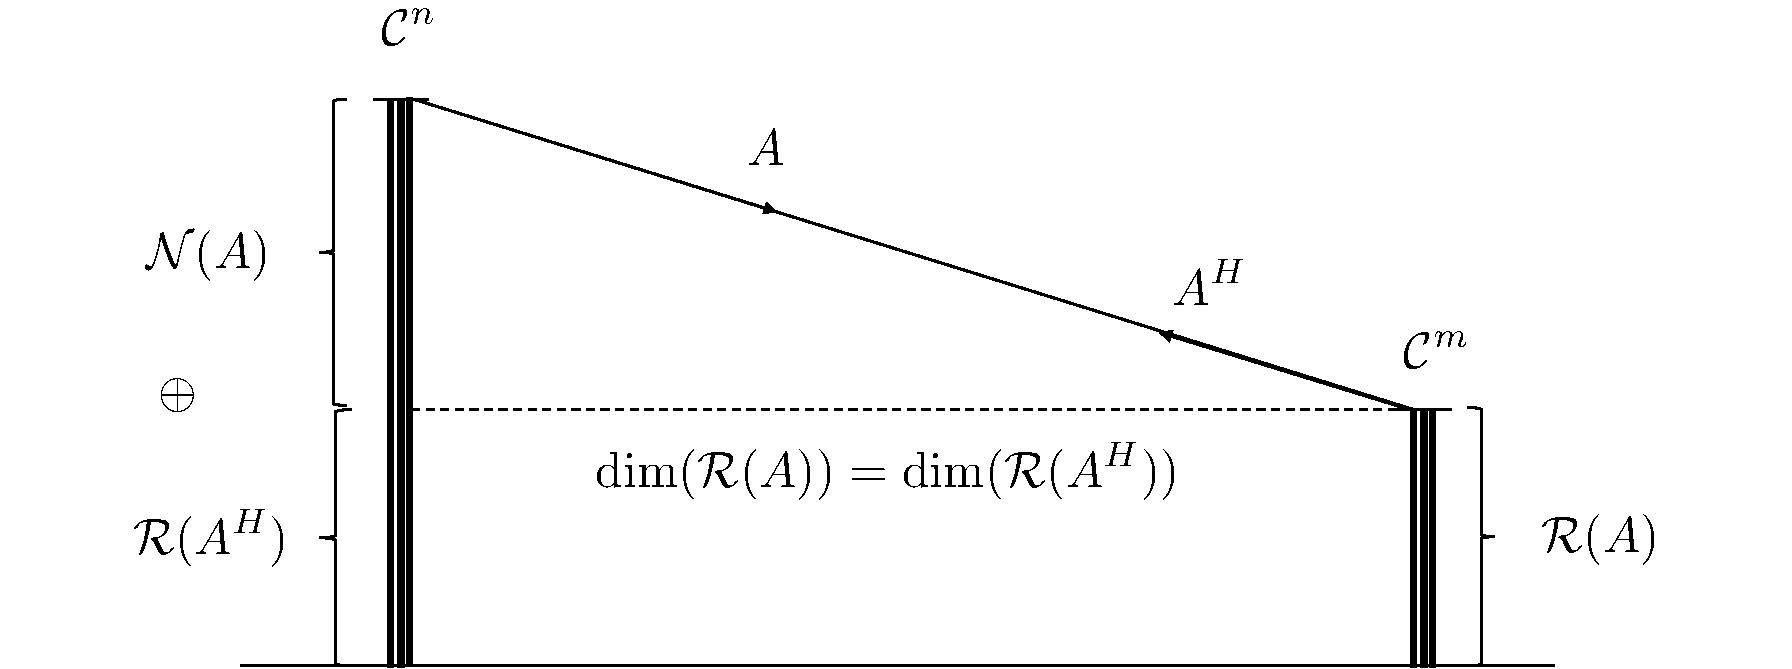
\includegraphics[width=\textwidth]{figures/chap4_min_norm}
	\end{center}
	
	We would like to solve $Ax = b$ note that since $x = x_r + x_n$ where $x_r \in \mathcal{R}(A^H)$ and $x_n \in \mathcal{N}(A)$ and $\mathcal{N}(A) \neq \{0\}$ there are an infinite number of solutions (i.e. add any thing in $\mathcal{N}(A)$ to a solution).  
	The minimum norm solution will be the element of $\mathcal{R}(A^H)$ that satisfies $Ax_r = b$.
\end{frame}

%----------------------------------
\begin{frame}\frametitle{Right Inverse: Min-norm Solution, cont.}
	\[ x_r \in \mathcal{R}(A^H) \Rightarrow x_r = A^Hy \text{ where } y \in \mathbb{C}^m \]
	so we need to solve
	\[ (\underset{m\times n}{A}\underset{n\times m}{A^H})\underset{m\times 1}{y} = \underset{m \times 1}{b} \]
	Since $rank(A) = rank(AA^H) = m$, $(AA^H)^{-1}$ exists.
	\[ \Rightarrow y = (AA^H)^{-1}b \]
	\[ \Rightarrow \fbox{ $x_r = A^H(AA^H)^{-1}b$ } \]
	Note that this is the same solution as
		\begin{mini*}|s|
		{}{\norm{x}_2}{}{}
		\addConstraint{Ax = b}	
		\end{mini*}
\end{frame}

%----------------------------------
\begin{frame}\frametitle{Right and Left Inverses}
	\begin{lemma}
		If $A\in\mathbb{C}^{m\times n}$ where $m>n$ and $A$ is full rank, then 	$ (A^HA)^{-1}A^H $ is a left inverse of $A$.
	\end{lemma}
	\begin{proof}
		$\qquad\qquad\qquad (A^HA)^{-1}A^HA = I_n$
	\end{proof}
	\begin{lemma}
		If $A\in\mathbb{C}^{m\times n}$ where $m<n$ and $A$ is full rank, then 	$A^H(AA^H)^{-1}b $ is a right inverse of $A$.
	\end{lemma}
	\begin{proof}
		$\qquad\qquad\qquad AA^H(AA^H)^{-1} = I_m$
	\end{proof}
	
	\begin{itemize}
		\item Both are examples of pseudo-inverses.
		\item $A^H(AA^H)^{-1}$ is called the Moore-Penrose pseudo-inverse.  
		\item In Matlab type \texttt{pinv(A)}.
	\end{itemize}
\end{frame}

%%%%%%%%%%%%%%%%%%%%%%%%%%%%%%%%%%%%%%%%%%%%%%%%%%%%%%%%%%%%%%%%%
\section{Matrix Condition Number}
\frame{\sectionpage}

%----------------------------------
\begin{frame}\frametitle{Matrix Condition Number}
	\begin{itemize}
	\item 	Suppose that $A \in \mathbb{C}^{n \times n}$ is full rank and $A^{-1}$ is to be computed numerically.  How reliable is the computation?
	\item $Ax = b$ can be written as 
		\[
			\begin{pmatrix}
   	 			a_{11} & \cdots & a_{1n}\\
    			\vdots & \ddots & \vdots\\
    			a_{n1} & \cdots & a_{nn}
    		\end{pmatrix}
    		\begin{pmatrix}
    			x_1 \\ \vdots \\ x_n
    		\end{pmatrix}
			=
			\begin{pmatrix}
				b_1 \\ \vdots \\ b_n	
			\end{pmatrix}
		\]
	\item Therefore, the solution $x$ is the intersection of $n-$ hyperplanes:
		\begin{align*}
		a_{11}x_1 + \ldots + a_{1n}x_n &= b_1\\
		\vdots\\
		a_{n1}x_1 + \ldots + a_{nn}x_n &= b_n
		\end{align*}
	\end{itemize}
\end{frame}

%----------------------------------
\begin{frame}\frametitle{Matrix Condition Number, cont.}
	\begin{itemize}
		\item The problem comes when these hyperplanes are almost parallel.
		\item In two dimensions we have two lines
			\begin{align*}
				a_{11}x_1 + a_{12}x_2 &= b_1\\
				a_{21}x_1 + a_{22}x_2 &= b_2
			\end{align*}
			which can be rewritten as
			\begin{align*}
  				x_2 &= -\frac{a_{11}}{a_{12}}x_1 + \frac{b_1}{a_{12}}\\
  				x_2 &= \underbrace{-\frac{a_{21}}{a_{22}}}_{\text{slope}}x_1 + \underbrace{\frac{b_2}{a_{22}}}_{\text{x-intercept}} 
			\end{align*}
	\end{itemize}
\end{frame}

%----------------------------------
\begin{frame}\frametitle{Matrix Condition Number, cont.}
	\begin{center}
		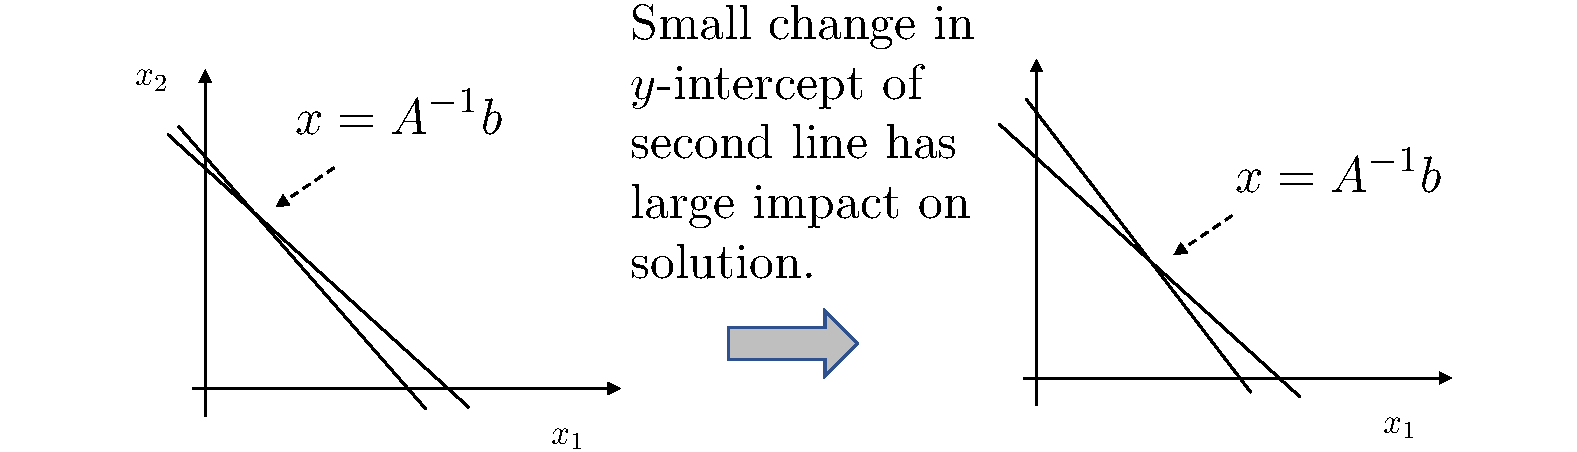
\includegraphics[width=\textwidth]{figures/chap4_condition_number}
	\end{center}
	If the two lines are almost parallel then small changes in the slope or $x_2$-intercept of either line will result in large changes in $x = A^{-1}b$.
\end{frame}

%----------------------------------
\begin{frame}\frametitle{Matrix Condition Number, cont.}
	\begin{itemize}
		\item Since computers must represent numbers to finite precision, representation errors could significantly change the numerical solution to the equation $Ax = b$.
		\item The condition number quantifies this effect.
	\end{itemize}
	
	\begin{definition}
		The condition number of a square matrix is defined to be
		\[ \mathcal{K}(A) = \norm{A }\norm{A^{-1} } \]
		where $\norm{\cdot }$ is an induced matrix norm usually taken to be the induced 2-norm.
	\end{definition}
\end{frame}

%----------------------------------
\begin{frame}\frametitle{Matrix Condition Number: Derivation}
	\begin{itemize}
		\item Given the two equations $Ax = b$ and $(A + \epsilon E)x = b$ where $\epsilon E$ is a ``small'' perturbation of $A$ (introduced by finite machine precision of $A$)
		\item Let $x_0 = A^{-1}b$ and
			\begin{align*}
				x_E &= (A + \epsilon E)^{-1}b\\
				&= [A(I + \epsilon A^{-1}E)]^{-1}b\\
				&= (I+\epsilon A^{-1}E)^{-1}A^{-1}b \\
				&= \underbrace{(I+\epsilon A^{-1}E)^{-1}}_{\text{perturbation}}x_0
			\end{align*}
	\end{itemize}
\end{frame}

%----------------------------------
\begin{frame}\frametitle{Matrix Condition Number: Derivation, cont.}
	Using the Neumann expansion gives
	$(I+\epsilon A^{-1}E)^{-1} = \displaystyle \sum_{i=0}^{\infty} (-\epsilon A^{-1} E)^i$.  Therefore
	\begin{align*}
		x_E &= (I+\epsilon A^{-1}E)^{-1}A^{-1}b \\ 
		&=(I - \epsilon A^{-1} E)A^{-1}b + O(\norm{\epsilon E }^2x_0)\\
		&= A^{-1}b - \epsilon A^{-1}EA^{-1}b + O(\norm{\epsilon E }^2x_0)\\
		&= x_0 - \epsilon A^{-1}Ex_0 + O(\norm{\epsilon E }^2x_0)
	\end{align*}
	Therefore
	\[\underbrace{\displaystyle\frac{\norm{x_E-x_0 }}{\norm{x_0 }}}_{\text{relative change in the solution}} \leq \underbrace{\epsilon\norm{A^{-1} }\norm{E }}_{\text{want to relate to relative change in $A$}}+O(\norm{\epsilon E }^2)  \]
\end{frame}

%----------------------------------
\begin{frame}\frametitle{Matrix Condition Number: Derivation, cont.}
	What is the relative change in $A$?
	\[\frac{  \norm{A - (A + \epsilon E) }}{  \norm{A }} = \frac{  \epsilon\norm{E }}{  \norm{A }} \defeq \rho\]
	Therefore
	\[
		\frac{ \norm{x_E - x_0 }}{\norm{x_0 }} \leq \rho \underbrace{\norm{A^{-1}}\norm{A } }_{\mathcal{K}(A)} + O(\norm{\epsilon E }^2) 
	\]
	
	The condition number $\mathcal{K}(A)$ relates (approximately) the relative change in $A$ to the relative change in the solution $x_0$.
\end{frame}

%----------------------------------
\begin{frame}\frametitle{Matrix Condition Number: Implication}
	\underline{Rule of Thumb:} \\
	If the solution is computed to $n$ digits then only
	\[ n - \log_{10} \mathcal{K}(A) \]
	can be considered to be accurate.
\end{frame}


%%%%%%%%%%%%%%%%%%%%%%%%%%%%%%%%%%%%%%%%%%%%%%%%%%%%%%%%%%%%%%%%%
\section{Schur Complement and the Matrix Inversion Lemma}
\frame{\sectionpage}

%----------------------------------
\begin{frame}\frametitle{Schur Complement}
	\begin{definition}
		Consider the partitioned matrix
		\[
		A = \begin{bmatrix} A_{11} & A_{12} \\ A_{21} & A_{22} \end{bmatrix}.
		\]	
		\begin{enumerate}
			\item When $A_{11}$ is non-singular, 
				\[ S_{ch}(A_{11}) \defeq A_{22} - A_{21}A_{11}^{-1}A_{12} \]
				is called the \underline{Schur Complement of $A_{11}$ in $A$}.
			\item When $A_{22}$ is non-singular, 
				\[ S_{ch}(A_{22}) \defeq A_{11} - A_{12}A_{22}^{-1}A_{21} \]
				is called the \underline{Schur Complement of $A_{22}$ in $A$}.
		\end{enumerate}
	\end{definition}
\end{frame}

%----------------------------------
\begin{frame}\frametitle{Schur Complement, cont.}
	\begin{lemma}
	When $A_{11}$ is nonsingular, $A$ is nonsingular if and only if $S_ch(A_{11})$ is nonsingular, in which case
	\[
	A^{-1} = \begin{bmatrix}
				A_{11}^{-1} + A_{11}^{-1}A_{12}S_{ch}^{-1}(A_{11})A_{21}A_{11}^{-1} &
				-A_{11}^{-1}A_{12}S_{ch}^{-1}(A_{11}) \\
				-S_{ch}^{-1}(A_{11})A_{21}A_{11}^{-1} &
				S_{ch}^{-1}(A_{11})
 			 \end{bmatrix}
	\]	
	\end{lemma}
	\begin{lemma}
	When $A_{22}$ is nonsingular, $A$ is nonsingular if and only if $S_ch(A_{22})$ is nonsingular, in which case
	\[
	A^{-1} = \begin{bmatrix}
				S_{ch}^{-1}(A_{22}) &
				-S_{ch}^{-1}(A_{22})A_{12}A_{22}^{-1} \\
				-A_{22}^{-1}A_{12}S_{ch}^{-1}(A_{22}) &
				A_{22}^{-1} + A_{22}^{-1}A_{21}S_{ch}^{-1}(A_{22})A_{12}A_{22}^{-1} 
 			 \end{bmatrix}
	\]	
	\end{lemma}
	\begin{proof}
	By direct manipulation.	
	\end{proof}
\end{frame}

%----------------------------------
\begin{frame}\frametitle{Matrix Inversion Lemma}
	\begin{lemma}[Matrix Inversion Lemma]
		If $A\in\mathbb{R}^{n\times n}$ and $R\in\mathbb{R}^{m\times m}$ are invertible, and $X\in\mathbb{R}^{n\times m}$ and $Y\in\mathbb{R}^{m\times n}$ then
		\[ (A + X R Y)^{-1} = A^{-1} - A^{-1}X(R^{-1}+YA^{-1}X)^{-1}YA^{-1} \]
	\end{lemma}
	\begin{proof}  Equate the $(2,2)$ elements of $A^{-1}$ in the previous slide, and re-label matrices.	
	\end{proof}
	
\end{frame}

%----------------------------------
\begin{frame}\frametitle{Matrix Inversion Lemma, cont.}
	\begin{itemize}
	\item 	A special case of this matrix inversion lemma is the formula
		\[ 
		(A + xy^H)^{-1} = A^{-1} - \frac{A^{-1}xy^H A^{-1}}{1 + y^H A^{-1}x} 
		\]
		where $x$ and $y$ are vectors.
	\item Sylvester's inequality gives
		\[
		rank(x)+rank(y) - 1 \leq rank(xy^H) \leq min(rank(x),rank(y)).
		\]
		But 
		\begin{align*}
			rank(x)+rank(y) - 1	&= 1 \\
			min(rank(x),rank(y)) &= 1
		\end{align*}
	\item Therefore $rank(xy^H) = 1$
	\end{itemize}
\end{frame}


%%%%%%%%%%%%%%%%%%%%%%%%%%%%%%%%%%%%%%%%%%%%%%%%%%%%%%%%%%%%%%%%%
\section{Recursive Least Squares Filtering}
\frame{\sectionpage}

%----------------------------------
\begin{frame}\frametitle{Least Squares Filtering Problem}
	\begin{figure}
		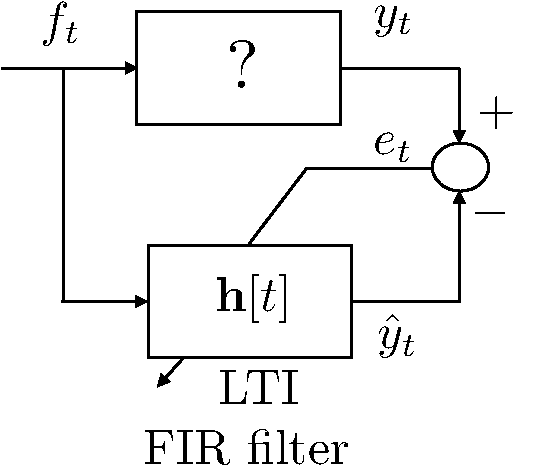
\includegraphics[width=0.5\textwidth]{figures/chap4_rls}	
	\end{figure}
	
	{\bf Problem Statement:}  Given the input data $f_t$ and $y_t$, find the FIR filter coefficients $\hbf[t]$ that minimize the running least squared error $e_t$.
	
\end{frame}



%----------------------------------
\begin{frame}\frametitle{Least Squares Filtering Problem}
	\begin{definition}[Least Squares Filtering Problem]
		Given the filter
		\[ \hat{y}_t = \sum_{i=1}^m h_i f_{t-i} \]
		where the inputs $f_t$ are known and we measure the actual outputs $y_t$, 
		find the coefficients $h_i$ such that the mean squared error 
		\[
		E = \sum_{i=1}^m \left( y_i-\hat{y}_i \right)^2
		\]
		is minimized.
	\end{definition}
\end{frame}

%----------------------------------
\begin{frame}\frametitle{Batch Least Squares Filtering}
	If we assume $f_t = 0, t \leq 0$ we get
	{\footnotesize
	\[
		\begin{pmatrix}
	 		y_1\\
 	   		y_2\\
 	   		\vdots\\
 	   		y_N
 	   	\end{pmatrix}
 	   	=
 	   	\begin{pmatrix}
   	  		f_1 & 0 & \cdots & \cdots & 0\\
  	  		f_2 & f_1 & 0 & \cdots & 0\\
    		\vdots & & & \ddots\\
    		f_m & f_{m-1} & \cdots & \cdots & f_1 \\
    		f_{m+1} & f_m & f_{m-1} & \cdots & f_2 \\
    		\vdots & & & \ddots \\
    		f_N & f_{N-1} & \cdots & \cdots & f_{N-m+1}
    	\end{pmatrix}
    	\begin{pmatrix}
    		h_1 \\
    		h_2 \\
    		\vdots\\
    		h_m
    	\end{pmatrix}
	\]
	}
\end{frame}

%----------------------------------
\begin{frame}\frametitle{Batch Least Squares Filtering, cont.}
	Define
	\begin{align*}
		\qbf_i &= \begin{pmatrix} f_i & f_{i-1} & \dots f_{i-m+1} \end{pmatrix}^H \\
		\ybf_N &= \begin{pmatrix} \bar{y}_1 & \bar{y}_2 & \dots \bar{y}_N \end{pmatrix}^H \\
		\hbf[N] &= \begin{pmatrix} \bar{h}_1[N] & \bar{h}_2[N] & \dots \bar{h}_m[N] \end{pmatrix}^H \\
		A_N &= \begin{pmatrix} \qbf^H_1 \\ \vdots \\ \qbf^H_m \end{pmatrix},
	\end{align*}
	then the least squares problem reduces to
	\[ 
		\ebf_N = \ybf_N - \underbrace{A_N \hbf[N]}_{\hat{\ybf}_N}
	\] 
	where $\ebf_N$ is the error to be minimized.  From the projection theorem, $\norm{\ebf}_2$ is minimized when
	\[
		\underset{m\times 1}{\hbf[N]} = (\underset{m \times N}{A^H_N} \underset{N \times m}{A_N)}^{-1}\underset{m\times N}{A^H_N}\underset{N\times 1}{\ybf_N}. 
	\]
\end{frame}

%----------------------------------
\begin{frame}\frametitle{Batch Least Squares Filtering}
	\begin{itemize}
		\item Note that the size of $y_N$ and $A_N$ grow linearly with time $N$.  
		\item Therefore, each time step requires more computation than the last step.  This is obviously problematic as $N\to\infty$.  
		\item For some $N$, batch least squares is no longer a real-time algorithm.
		\item Note that at time $N+1$ the data include new samples, but includes all of the data available at time $N$.
	\end{itemize}
	
	\vspace{1cm}
	
	{\color{red} ???  Is is possible to design an algorithm with fixed computational cost at each time step, that produces the same least squares solution?}
\end{frame}

%----------------------------------
\begin{frame}\frametitle{Recursive Least Squares Filtering}
	Define
	\begin{align*}
		\qbf_t &= \begin{pmatrix} f_i & f_{i-1} & \dots f_{i-m+1} \end{pmatrix}^H \\
		\ybf_t &= \begin{pmatrix} \bar{y}_1 & \bar{y}_2 & \dots \bar{y}_t \end{pmatrix}^H \\
		\hbf[t] &= \begin{pmatrix} \bar{h}_1[t] & \bar{h}_2[t] & \dots \bar{h}_m[t] \end{pmatrix}^H \\
		A_t &= \begin{pmatrix} \qbf^H_1 \\ \vdots \\ \qbf^H_t\end{pmatrix}.
	\end{align*}
	Then at time $t$ we have $\ebf_t = \ybf_t - A_t \hbf[t]$.  From the projection theorem, the error is minimized when
	\[
		\hbf[t] = (A^H_t A_t)^{-1} A_t^H \ybf_t.
	\]
\end{frame}

%----------------------------------
\begin{frame}\frametitle{Recursive Least Squares Filtering, cont.}
	Let 
	\begin{align*}
		R_{t-1} &\defeq A^H_{t-1} A_{t-1} 
		     = \begin{pmatrix}\qbf_1 & \cdots & \qbf_{t-1}\end{pmatrix} \begin{pmatrix} \qbf^H_1 \\ \vdots \\ \qbf^H_{t-1} \end{pmatrix} \\
		    &= \sum_{i=1}^{t-1} \qbf_i \qbf^H_i
	\end{align*}
	be the associated Grammian when there are $t-1$ samples.  
	
	\vfill
	
	Suppose that we receive new data $q_t$ and $y_t$ at time $t$.
	
	\vfill
	
	Then 
	\begin{align*}
		R_t &= \sum_{i=1}^{t} \qbf_i \qbf^H_i \\
		    &= \sum_{i=1}^{t-1} \qbf_i \qbf^H_i  + \qbf_t \qbf_t^H \\
		    &= R_{t-1} + \qbf_t \qbf_t^H.
	\end{align*}
\end{frame}

%----------------------------------
\begin{frame}\frametitle{Recursive Least Squares Filtering, cont.}
	In the solution $\hbf_t = (A_t^H A_t)^{-1} A_t^H \ybf_t$, we need $R_t^{-1} \defeq (A_t^H A_t)^{-1}$.
	
	Note that 
		\[R_t^{-1} = (\underbrace{R_{t-1}}_{A} + \underbrace{q_t}_{X}\underbrace{}_{R=1}\underbrace{q_t^H}_{Y})^{-1}\] 
	and recall the matrix inversion lemma:
		\[ (A + XRY)^{-1} = A^{-1} - A^{-1}X(R^{-1}+YA^{-1}X)^{-1}YA^{-1} \]
	Therefore
		\[R_t^{-1} = R_{t-1}^{-1} - R^{-1}_{t-1} \qbf_t(1 + \qbf_t^H R^{-1}_{t-1} \qbf_t)^{-1}\qbf_t^H R^{-1}_{t-1}.\]
\end{frame}

%----------------------------------
\begin{frame}\frametitle{Recursive Least Squares Filtering, cont.}

	Defining $P_t = R_t^{-1}$ gives
		\[
		P_t = P_{t-1} - \frac{P_{t-1} \qbf_t \qbf_t^H P_{t-1}}{1 + \qbf_t^H P_{t-1} \qbf_t}.
		\]
	Define the (Kalman) gain as
		\[ 
		\kbf_t = \frac{P_{t-1} \qbf_t}{1 + \qbf_t^H P_{t-1} \qbf_t}
		\]
	Then
	\[ 
	P_t = P_{t-1} - \kbf_t \qbf_t^H P_{t-1}. 
	\]
	Note that we have found a fixed computational scheme to update
	\[
	P_t = (A_t^H A_t)^{-1} 
	\]
	using old data $P_{t-1}$ and new data $\qbf_t$.
\end{frame}


%----------------------------------
\begin{frame}\frametitle{Recursive Least Squares Filtering, cont.}
		In the solution $\hbf[t] = (A_t^H A_t)^{-1} A_t^H \ybf_t$, we have found a clever way to update $P_t=(A_t^H A_t)^{-1}$ recursively.  Define
		\[
		\zbf_t \defeq A_t^H \ybf_t.
		\]
		We need a recursive update for $\zbf_t$.
		
		Toward that end note that
		\begin{align*}
			\zbf_t &= A_t^H \ybf_t \\
			 	&= \sum_{i=1}^t \qbf_i y_i \\
			 	&= \sum_{i=1}^{t-1} \qbf_i y_i + \qbf_t y_t \\
				&= \zbf_{t-1} + \qbf_t y_t
		\end{align*}
\end{frame}

%----------------------------------
\begin{frame}\frametitle{Recursive Least Squares Filtering, cont.}
	Therefore
	\begin{align*}
		\hbf_t	&= (A_t^H A_t)^{-1} A_t^H \ybf_t \\
				&= P_t \zbf_t \\
				&= (P_{t-1} - \kbf_t \qbf_t^H P_{t-1})(\zbf_{t-1} + \qbf_t y_t)\\
				&= P_{t-1} \zbf_{t-1} - \kbf_t \qbf_t^H P_{t-1} \zbf_{t-1} + P_{t-1} \qbf_t y_t - \kbf_t \qbf_t^H P_{t-1} \qbf_t y_t\\
				&= \hbf_{t-1} - \kbf_t \qbf_t^H \hbf_{t-1} + \underbrace{\left( P_{t-1}-\kbf_t \qbf_t^H P_{t-1} \right)}_{P_t} \qbf_t y_t \\
				&= \hbf_{t-1} + \kbf_t(y_t - \qbf_t^H \hbf_{t-1}) \\
		\implies \hbf_t &= \hbf_{t-1} + \kbf_t(y_t - \hat{y}),
	\end{align*}
	where we have used the fact that $P_t q_t = \kbf_t$.

	Note that $\hat{y}_t = \qbf_t^H \hbf_{t-1}$ is the predicted output, and $e_t=y_t-\hat{y}_t$ is the quantity that is being minimized.
\end{frame}

%----------------------------------
\begin{frame}\frametitle{Summary: Recursive Least Squares Filtering}
	At time $t=0$ initialize algorithm with
	\begin{align*}
		P_0 &= \alpha I, \text{~where $\alpha>0$ is a large number} \\
		\hbf_0 &= 0.
	\end{align*}
	At time $t$, get $y_t$, $f_t$, and compute $\qbf_t$ from $f_t$.  Update the least squares estimate using  
	\begin{align*}
  		\kbf_t &= \frac{P_{t-1} \qbf_t}{1 + \qbf_t^H P_{t-1} \qbf_t} \\
  		P_t &= P_{t-1} - \kbf_t \qbf_t^H P_{t-1} \\
  		\hbf_t &= \hbf_{t - 1} + \kbf_t (y_t - \qbf_t^H \hbf_{t-1}).
	\end{align*}
This is equivalent to a discrete time Kalman filter with stationary dynamics.
	
\end{frame}

\end{document}
